%--------------------------------------------------------------------------------------------------
\chapter{Umsetzung des Konzepts mit Hilfe der Unity Engine}\label{cha:Umsetzung}
In diesem Kapitel wird die Umsetzung des Menschmodells und der Interaktionsschnittstelle mit Hilfe der Entwicklungsumgebung Unity Engine vorgestellt. Daher gibt es zunächst eine Einführung in die verwendete Hardware und Software, bevor das Menschmodell und die Interaktionsschnittstelle genauer erläutert werden.
%--------------------------------------------------------------------------------------------------
\section{Verwendete Hardware}\label{sec:Hardware}

\subsection{VIVE Pro Brille, Wireless Set, Basisstationen und Controller}\label{sec:GrundHardware}
Für die Umsetzung dieses Projektes wurde die Virtual Reality Brille \textbf{VIVE Pro} (Vgl. Abbildung \ref{fig:ViveproKit}) vom Hersteller HTC verwendet, da sie eine der leistungsstärksten Brillen auf dem Markt ist. Zu den Stärken dieser Brille gehören das kontrastreiche OLED-Display, die sehr hohe Auflösung von 1440 x 1600 Pixeln pro Auge, eine Bildwiederholrate von 90Hz, ein Sichtfeld von 110 Grad und vor allem die Möglichkeit, die Brille mit Hilfe des \textbf{Vive Wireless Sets} (Vgl. Abbildung \ref{fig:WirelessKit}) kabellos zu verwenden. Es ist anzumerken, dass für das kabellose Verwenden dieser VR Brille eine Erweiterungskarte in den PC eingebaut werden muss, um einen speziellen Empfänger für die Signale der Brille anzuschließen. Des Weiteren muss ein Sender an der VR-Brille angebracht werden, welcher mit dem am PC angeschlossenen Empfänger kommuniziert und durch einen mobilen Akku mit Strom versorgt wird. Der mitgelieferte mobile Akku ermöglicht einen kabellosen Einsatz der VR Brille für bis zu sechs Stunden (Vgl. Abbildung \ref{fig:WirelessKit}) \cite{28}.
Die Brille zu verwenden zu können erfordert mindesten zwei der sogenannten \textbf{SteamVR 2.0 Basisstationen} (Vgl. Abbildung \ref{fig:ViveproKit}), welche dem Bediener, in Kombination mit dem Vive Wireless Set, eine enorme Bewegungsfreiheit ermöglichen. Beim Einsatz von zwei solcher Basisstationen ist eine Raumgröße von bis zu 5m x 5m, also 25m² möglich. Es ist sogar möglich, bis zu vier solcher Basisstationen zu Verwenden und somit eine Raumgröße von bis zu 10m x 10m, also 100m² zu unterstützen \cite{28}.
Ein weiteres notwendiges Zubehör der Brille sind die beiden \textbf{Controller} (Vgl. Abbildung \ref{fig:ViveproKit}), die es dem Bediener ermöglichen mit der virtuellen Umgebung zu interagieren. Beide Controller werden, wie die VR Brille, durch die Basisstationen im Raum geortet und liefern Informationen über ihre eigene Position und Ausrichtung im Raum. Zusätzlich verfügen beide Controller über jeweils fünf Tasten, welche mit eigenen Funktionalitäten versehen werden können. Es ist anzumerken, dass die Tasten alle unterschiedlich sind und daher für unterschiedliche Zwecke verwendet werden können \cite{29}.
\newline
Auf beiden Controllern befinden sich jeweils fünf Tasten \cite{29}:
\begin{itemize}
	\item Die erste dieser Tasten (Vorderseite, ganz unten) ist die Taste für das aufzurufen des Hauptmenüs und behält in der Regel diese Funktionalität bei.
	\item Die zweite Taste (Vorderseite, mittig) ist gleichzeitig ein berührungsempfindliches Trackpad. Dem 
	Entwickler steht es frei, ob er diese Taste als einfache Taste oder als Trackpad verwenden 
	möchte. Es ist sogar Möglich beide Funktionen gleichzeitig in einer Anwendung zu 
	unterstützen. Dadurch eröffnen sich viele Anwendungsmöglichkeiten für diese Taste.
	\item Die dritte Taste (Vorderseite, oben) ist wiederrum eine ganz einfache Taste und wird in den meisten 
	Anwendungen als eine Menü-Taste verwendet.
	\item Die Tasten links und rechts an der Außenseite des Controllers bilden eine zusammenhängende Taste, welche ausgelöst wird, wenn der Bediener den Controller fest mit der Hand drückt.
	\item Die Taste auf der Rückseite hat, genauso wie das Trackpad auf der Vorderseite, zwei 
	Einsatzmöglichkeiten. Sie kann einerseits als einfache Taste verwendet werden, andererseits 
	als berührungsempfindlicher Auslöser, da der Entwickler über die Software-Schnittstelle 
	auslesen kann, wie tief die Taste eingedrückt wurde, ähnlich wie bei einem Gaspedal in
	einem Auto.
\end{itemize}
\begin{figure}[h]
	\centering
	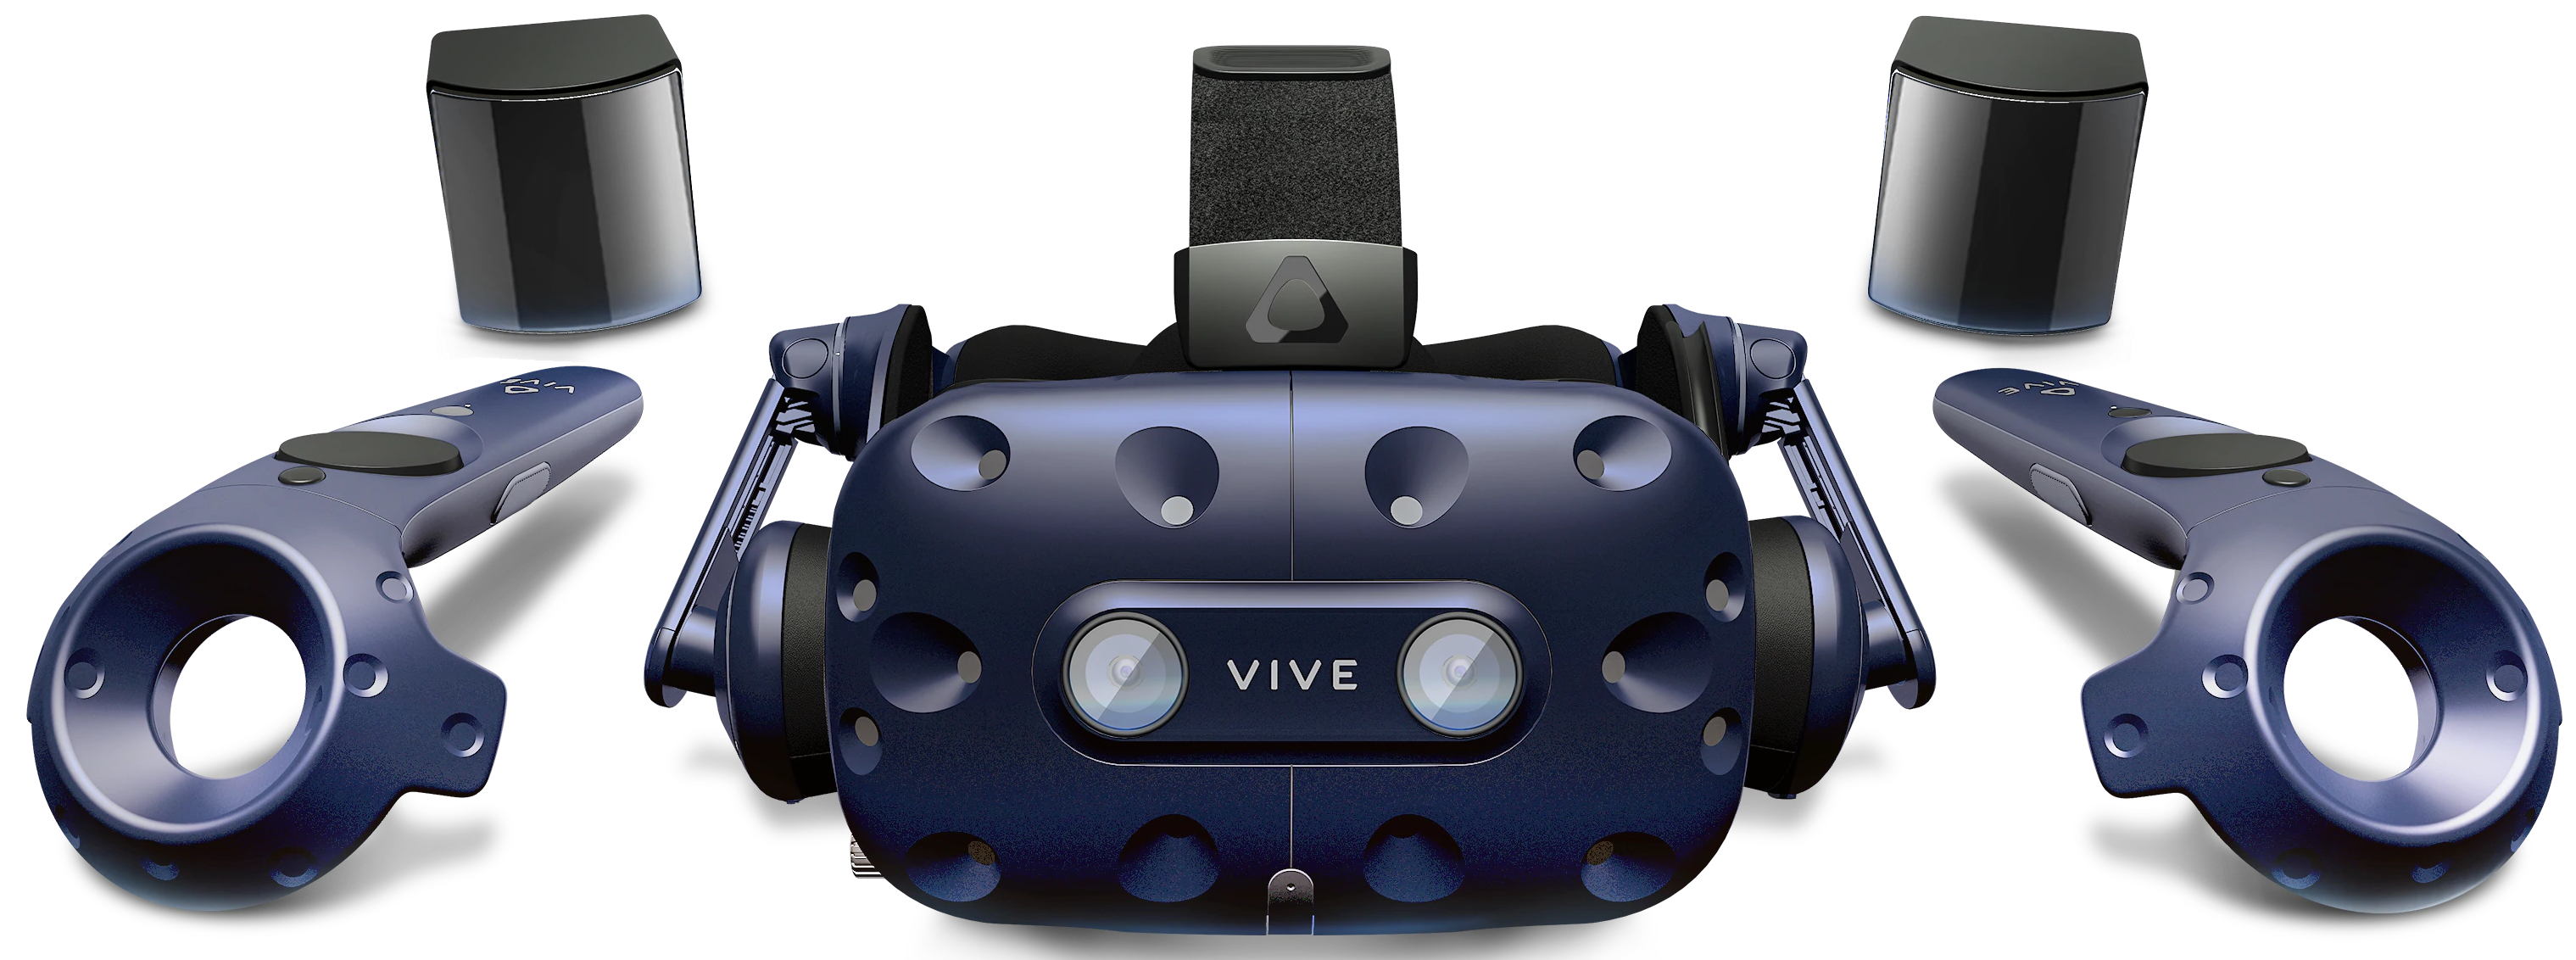
\includegraphics[width=0.6\linewidth]{Bilder/A26_Vivepro2}
	\caption{Die HTC VIVE Pro, die Controller und die Basisstationen \cite{A26}}
	\label{fig:ViveproKit}
\end{figure}
\begin{figure}[h]
	\centering
	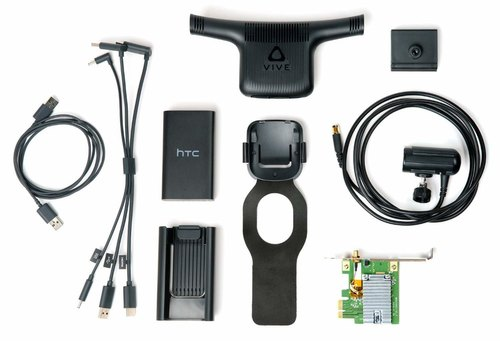
\includegraphics[width=0.4\linewidth]{Bilder/A27_WirelessKit}
	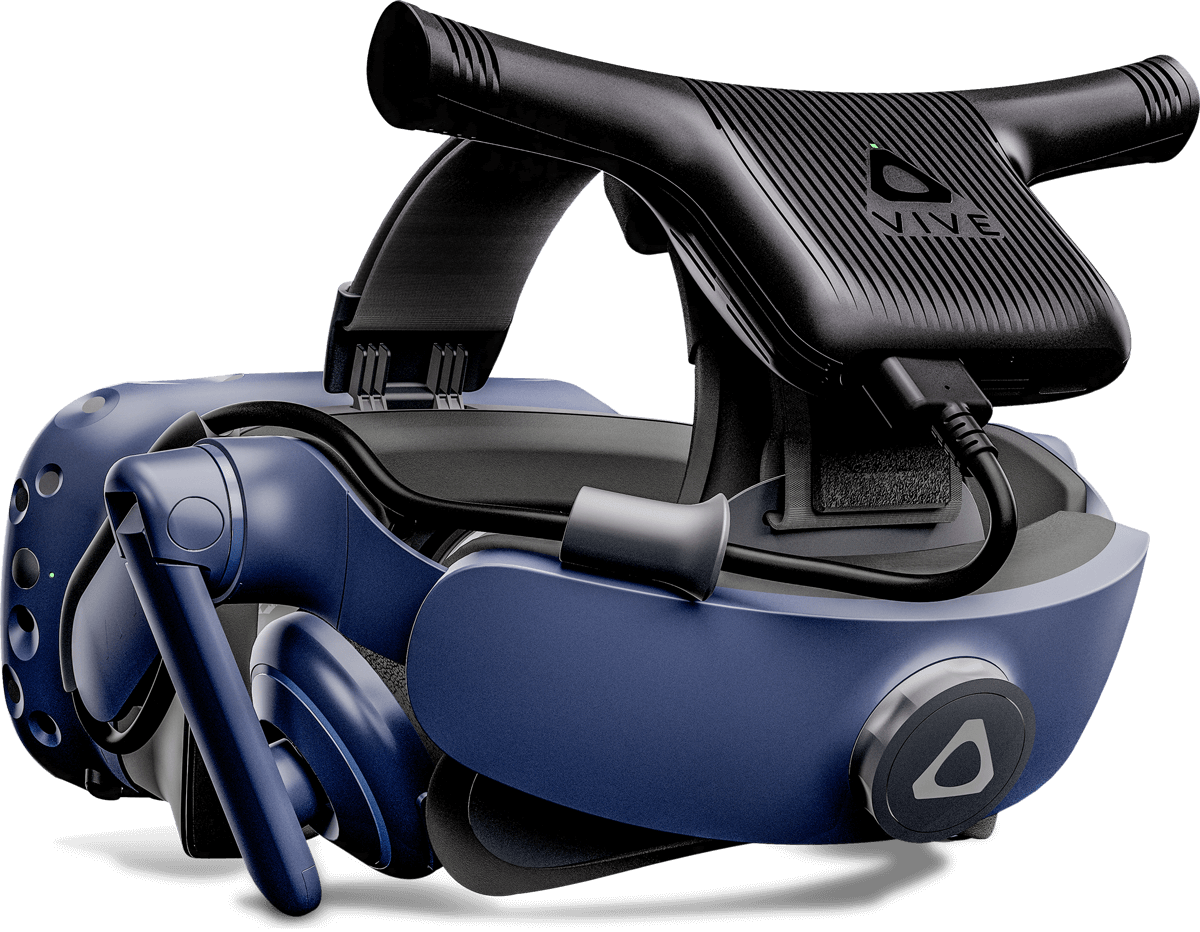
\includegraphics[width=0.32\linewidth]{Bilder/A28_Vive+Wireless}
	\caption{Das VIVE Wireless Set, inkl. Erweiterungskarte, Sender, Empfänger, Akku, etc. und die VR Brille mit angeschlossenem Sender \cite{A27,A28}}
	\label{fig:WirelessKit}
\end{figure}

\subsection{VIVE Tracker}\label{sec:TrackerVive}
Neben den außerordentlich guten technischen Spezifikationen der HTC VIVE Pro waren die \textbf{HTC VIVE Tracker} (Vgl. Abbildung \ref{fig:ViveTracker}) ein weiterer Grund, warum diese VR Brille zur Umsetzung dieser Arbeit ausgewählt wurde. Die VIVE Tracker werden genauso wie die VR Brille und die dazugehörigen Controller von den Basisstationen im raum geortet und liefern ebenfalls Informationen über ihre Position und Ausrichtung im Raum. Durch den kleinen Formfaktor können die Tracker an beliebigen Objekten befestigt werden, um die Bewegung dieser Objekte in der virtuellen Welt abzubilden \cite{30}.
\newline
\begin{figure}[h]
	\centering
	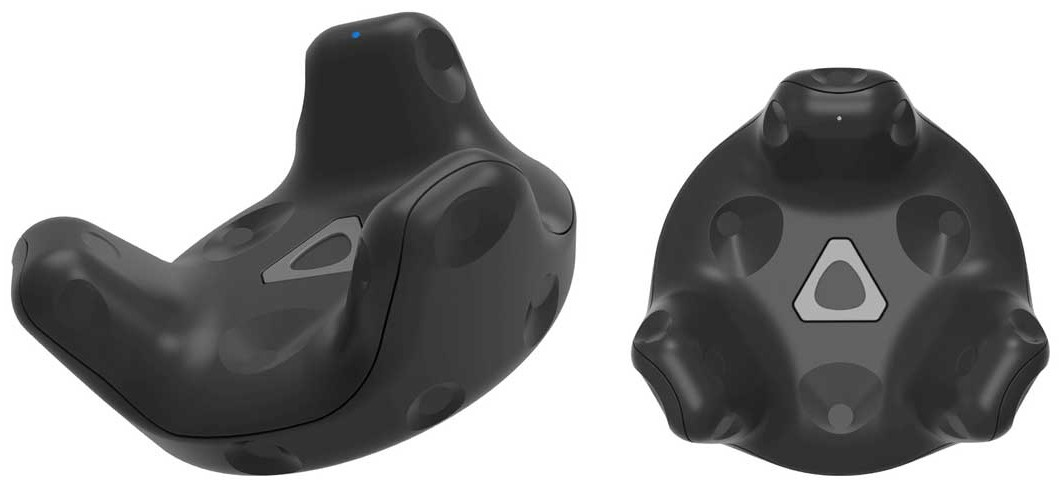
\includegraphics[width=0.6\linewidth]{Bilder/A29_ViveTracker}
	\caption{Die HTC VIVE Tracker \cite{A29}}
	\label{fig:ViveTracker}
\end{figure}

\subsection{Befestigungen für die Tracker}\label{sec:TrackerBefestigung}
Bei dieser Arbeit kamen die Tracker für die Ortung weiterer Körperteile zum Einsatz, da die Hände und der Kopf bereits mit Hilfe der Controller in den Händen und der VR Brille auf dem Kopf geortet werden können. Konkret kamen die Tracker für die Ortung der Füße, der Knie, des Beckens und der Ellenbogen zum Einsatz. Durch das Schraubgewinde auf der Unterseite lassen sich die Tracker einfach befestigen. Für die Befestigungen am Becken und an den Füßen wurde auf \textbf{fertige Halterungen} zurückgegriffen (Vgl. Abbildung \ref{fig:Mounts}). Für die Fixierung der Tracker an den Knien und an den Ellenbogen habe ich mir \textbf{eigene Halterungen} gebaut (Vgl. Abbildung \ref{fig:Mounts}). Für diese Halterungen wurden handelsübliche Knie- und Ellenbogenschoner verwendet, durch die ein Loch gebohrt wurde, um eine Schraube mit Hilfe einer Mutter zu fixieren. Durch das bereits erwähnte Schraubgewinde auf der Unterseite der Tracker, ließen diese sich einfach an diesen Schrauben befestigen.
\begin{figure}[h]
	\centering
	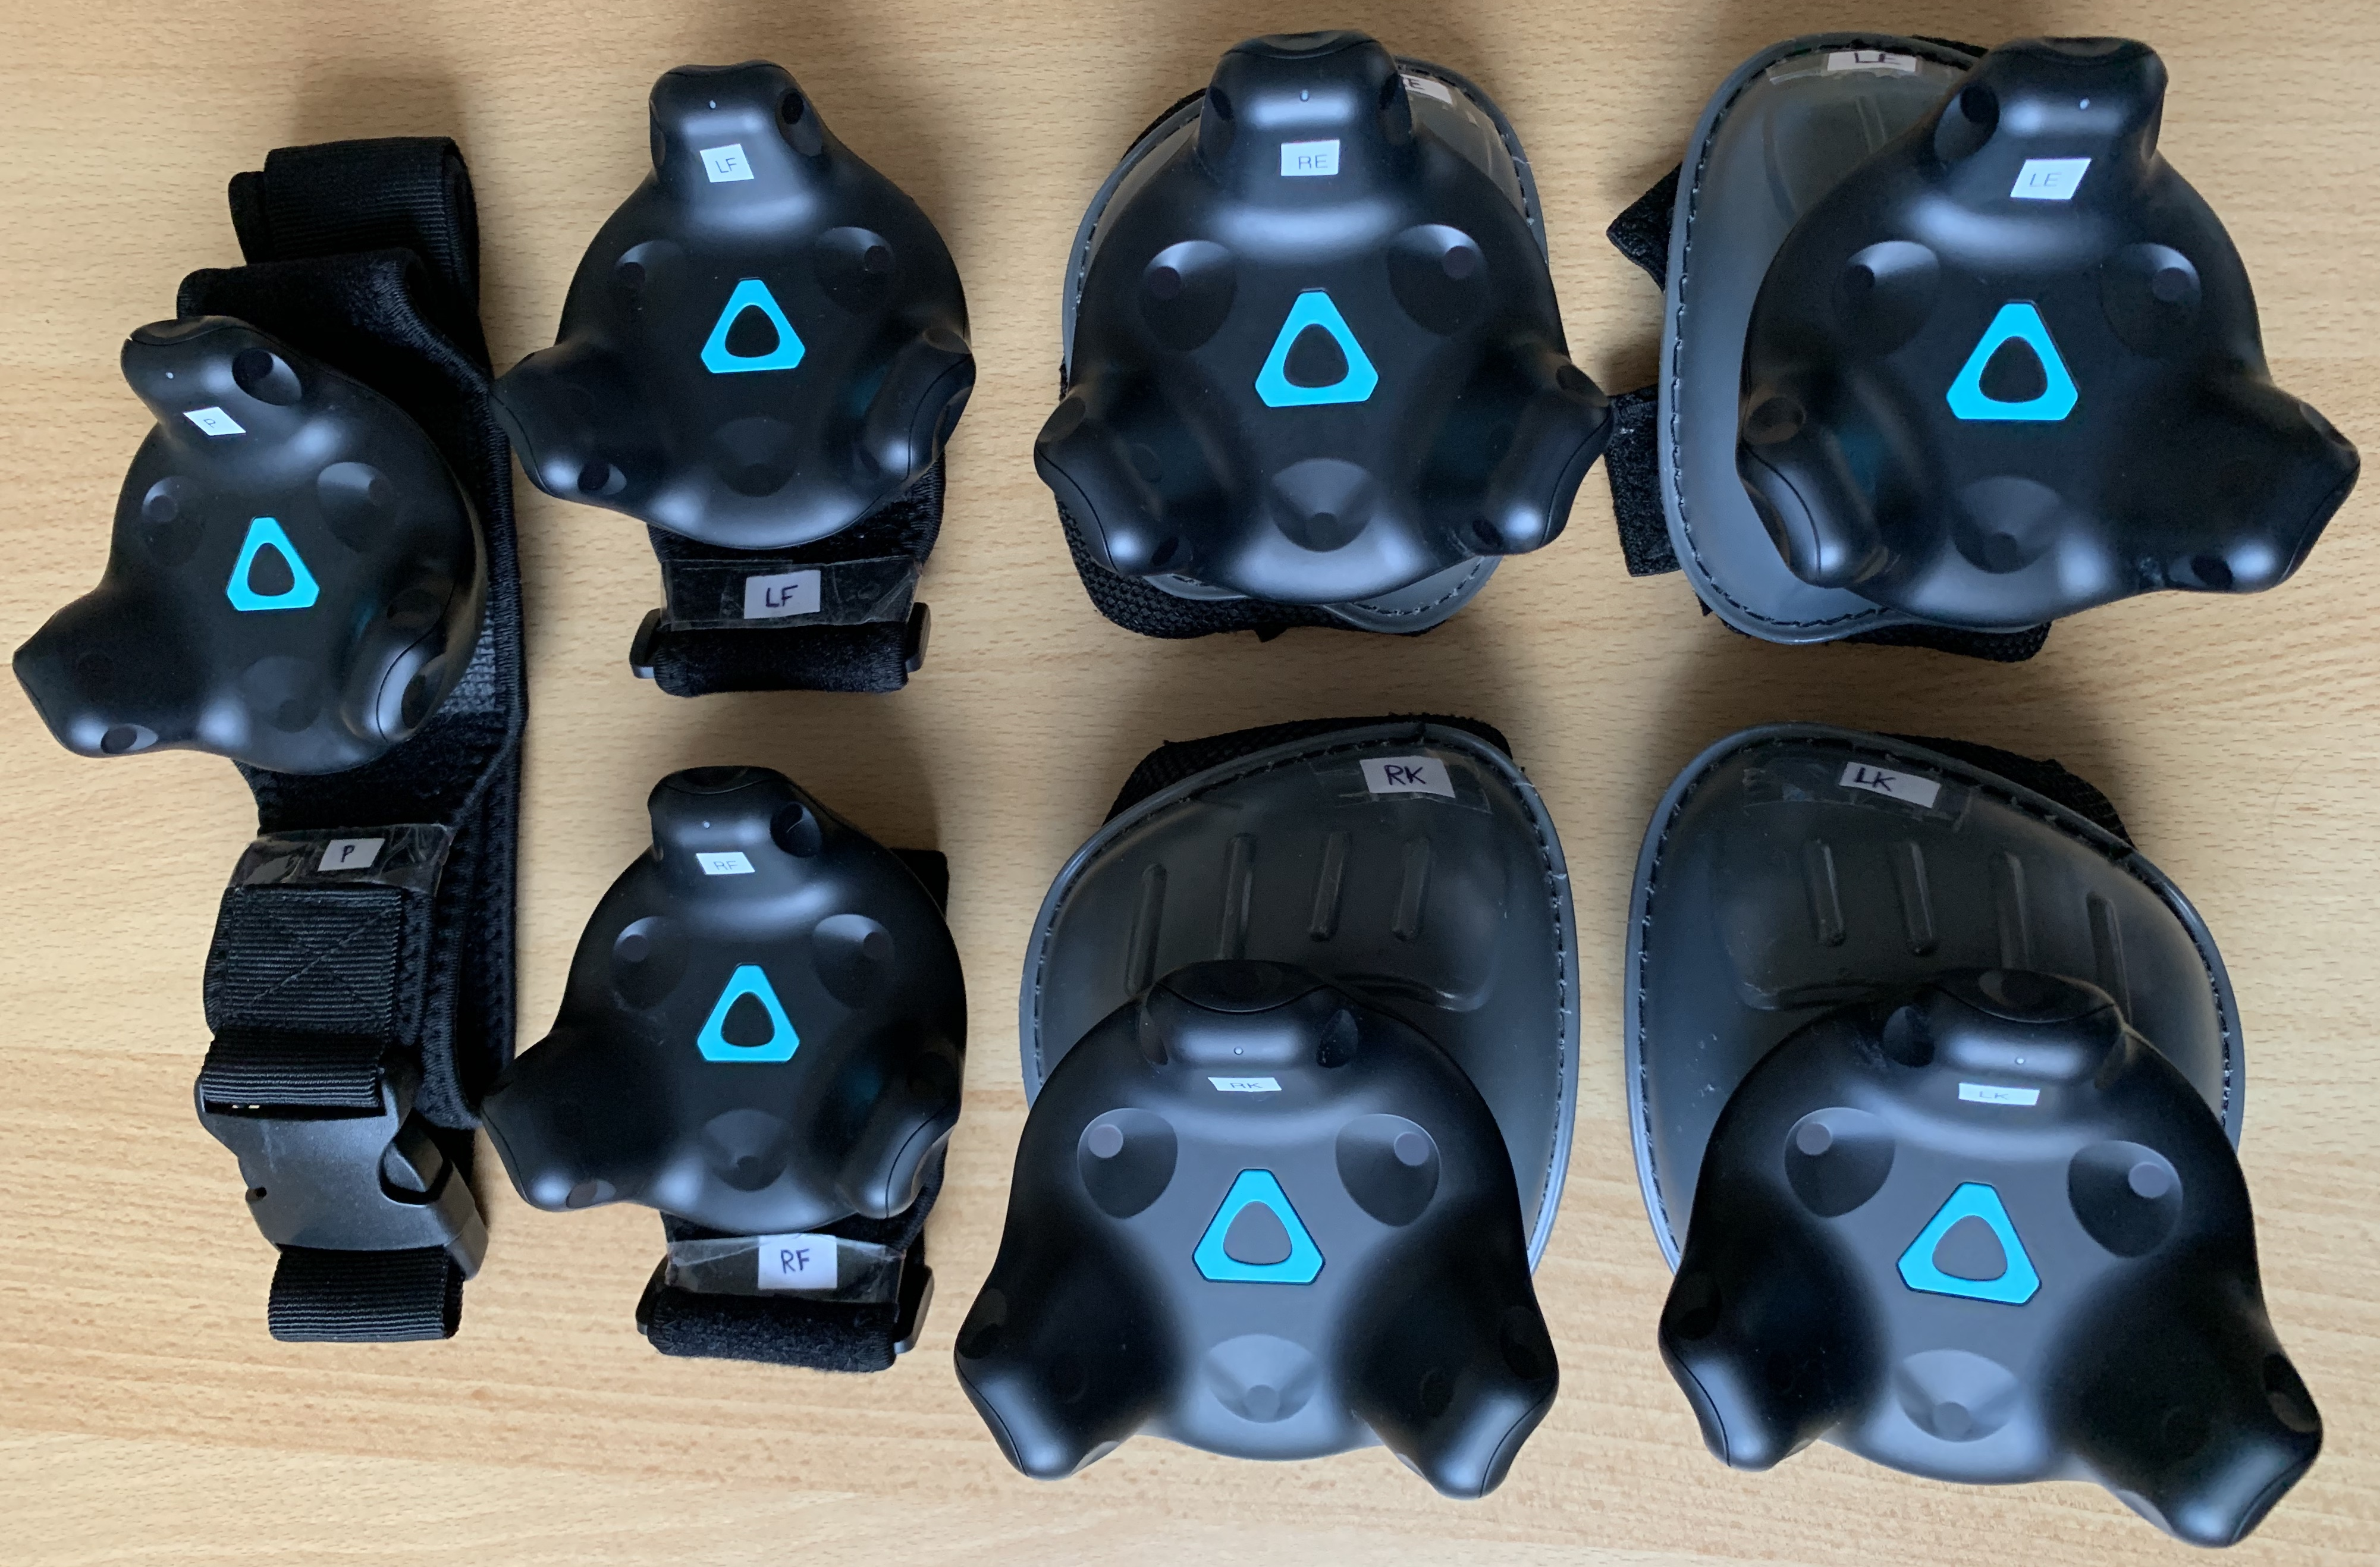
\includegraphics[width=0.8\linewidth]{Bilder/A32_Mounts}
	\caption{Die gekauften und eigenen Befestigungen für die Tracker, eigene Abbildung}
	\label{fig:Mounts}
\end{figure}
\newpage
%--------------------------------------------------------------------------------------------------
\section{Eingesetzte Software}\label{sec:Software}
Wie in Abbildung \ref{fig:CodeDarstellung} bereits angedeutet, kamen für die Umsetzung dieses Projekts verschiedene Anwendungen und Plugins zum Einsatz. Im Folgenden wird, neben den eingesetzten Anwendungen und Plugins, insbesondere die verwendete Entwicklungsumgebung Unity Engine genauer erläutert.

\subsection{VIVE Wireless Anwendung}\label{sec:VIVEWireless}
Die VIVE Wireless Anwendung (Vgl. Abbildung \ref{fig:VIVEWirelessSteamVR}) ist für die direkte Verbindung mit der VR Hardware verantwortlich. Wie bereits in Abbildung \ref{fig:WirelessKit} dargestellt, wird dafür im Computer eine Erweiterungskarte installiert, die es einem ermöglicht, den entsprechenden Empfänger für die Signale am PC anzuschließen. Der in Abbildung \ref{fig:WirelessKit} dargestellte, an der VR Brille montierte Sender, bildet das Gegenstück zu diesem Empfänger. Diese Erweiterung der Hardware, in Kombination mit der VIVE Wireless Anwendung und dem mobilen Akku, ermöglicht die kabellose Verwendung der VR Brille und somit die freie Bewegung des Bedieners im Raum.

\subsection{SteamVR Anwendung}\label{sec:SteamVR}
SteamVR (Vgl. Abbildung \ref{fig:VIVEWirelessSteamVR}) stellt eine weitere wichtige Anwendung im Kontext dieser Arbeit dar. Viele Anwendungen für VR Brillen, von unterschiedlichen Herstellern, sind auf die Schnittstelle der SteamVR Software ausgelegt. Das Gegenstück zu dieser Schnittstelle bildet das SteamVR Plugin, welches im weiteren Verlauf dieses Kapitels vorgestellt wird und nur für Entwickler relevant ist. Falls die VR Brille ohne das VIVE Wireless Set verwendet wird, wird diese über ein Kabel direkt mit dem PC und somit direkt mit der SteamVR Anwendung verbunden. Für diese Arbeit wurde jedoch das VIVE Wireless Set eingesetzt, somit wurde die VR Brille indirekt über die VIVE Wireless Anwendung mit der SteamVR Anwendung verbunden. Des Weiteren bringt die SteamVR Anwendung eine große Menge an Funktionalitäten mit sich. Dazu gehören beispielsweise die Möglichkeit, den Spielraum zu vermessen oder die Tastenbelegungen der Controller zu verändern. Zusätzlich bietet SteamVR eine Art Hauptmenü an, welches über die in Kapitel \ref{sec:Hardware} angesprochene Taste aufgerufen werden kann. Abschließend lässt sich sagen, dass SteamVR eine zentrale Schnittstelle bietet, mit der sich die VR Brille, die Controller, die Basisstationen und die Tracker verwalten lassen.
\begin{figure}[h]
	\centering
	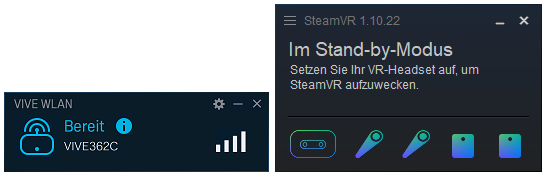
\includegraphics[width=0.8\linewidth]{Bilder/A33_VIVESteam}
	\caption{Die VIVE Wireless und SteamVR Anwendungen, eigene Abbildung}
	\label{fig:VIVEWirelessSteamVR}
\end{figure}

\subsection{Unity Engine Entwicklungsumgebung}\label{sec:UnitEngine}
Die Unity Engine ist eine 3D-Entwicklungsumgebung und wurde für die Umsetzung dieser Arbeit verwendet. Als Programmiersprache für diese Entwicklungsumgebung kommt die Sprache C\# zum Einsatz. Unity bietet den Vorteil, in einem Projekt mehrere Szenen (Umgebungen) aufsetzen und schnell zwischen diesen wechseln zu können. Des Weiteren können diese Szenen direkt in der Anwendung bearbeitet werden, wenn z.B. 3D-Modelle bearbeitet, hinzugefügt oder entfernt werden sollen. Außerdem bringt die Unity Engine eine Vielzahl von bereits eingebauten Funktionalitäten mit sich, die Entwicklern einiges an Arbeit ersparen können. So gibt es Beispielweise vorgefertigte Elemente für graphische Benutzeroberflächen oder sogar ein eingebautes Physiksystem, mit dem sich z.B. Kollisionen von Objekten leicht abfragen lassen können. Dank des eingebauten Asset Stores (Marktplatz), lassen sich in einem internen Marktplatz, aus einer großen Auswahl an Plugins, Erweiterungen, Texturen, Modellen, etc., beliebig viele Komponenten herunterladen und im eigenen Projekt einfügen. Aufgrund dessen lässt sich sagen, dass Unity als Entwicklungsumgebung den Entwicklern ermöglicht, Modularität in ihren Projekten umzusetzen.
Auch bei dieser Arbeit kamen Erweiterungen aus dem Asset Store zum Einsatz. Neben vereinzelten Texturen aus dem Asset Store, sind die wichtigsten Erweiterungen für diese Arbeit das SteamVR und das Final IK Plugin, welche im weiteren Verlauf dieses Kapitels genauer erläutert werden.
\newline\newline
Bevor die angesprochenen Plugins vorgestellt und die Umsetzung des Menschmodells und der Interaktionsschnittstelle erläutert werden, gibt es zunächst eine Einführung in den Aufbau der Unity Entwicklungsumgebung. Es ist anzumerken, dass das Projekt mit Hilfe der Version 2019.2.19f1 von Unity entwickelt wurde.
\begin{figure}[h]
	\centering
	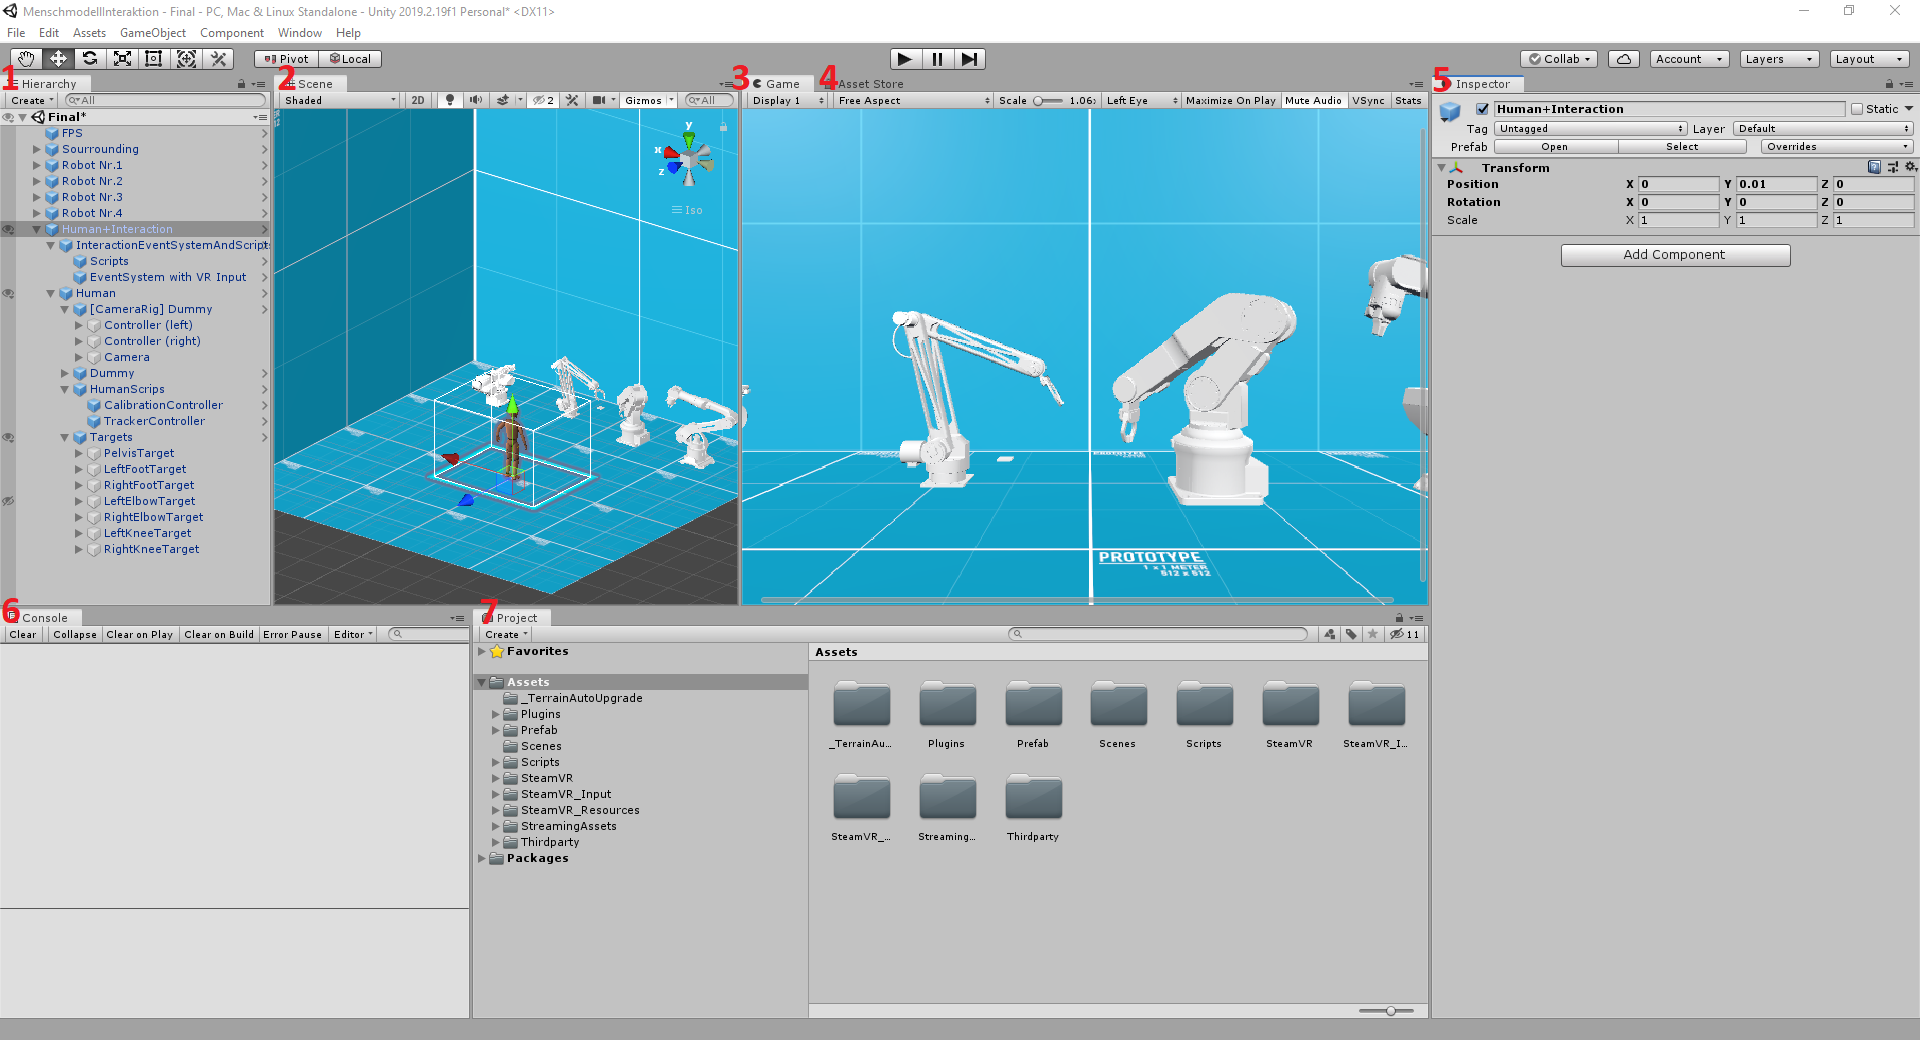
\includegraphics[width=1\linewidth]{Bilder/A47_UnityOverview2}
	\caption{Die Unity Entwicklungsumgebung, eigene Abbildung}
	\label{fig:UnityOverview}
\end{figure}
\newpage
\noindent Das Fenster der Entwicklungsumgebung besteht aus den Komponenten Hierarchy (Hierarchie), Scene (Szene), Game (Spiel), Asset Store (Marktplatz), Inspector (Inspektor), Console (Konsole) und Project (Projekt) (Vgl. Abbildung \ref{fig:UnityOverview}). Im weiteren Verlauf der Arbeit enthalten die Abbildungen die Nummer des Fensters in dem sie vorkommen (rote Zahl in der Abbildung).
\begin{enumerate}
	\item \textbf{Hierarchy (Hierarchie)} \\
	Mit Hilfe dieser Komponente enthält der Entwickler einen Überblick über die Objekte in der aktuellen Szene. Dies ermöglicht dem Entwickler Objekte hinzuzufügen, zu bearbeiten oder sogar zu entfernen. Wie in Abbildung \ref{fig:UnityOverview} zu erkennen ist, besteht die Szene der finalen Abgabe dieser Arbeit lediglich aus dem FPS Zähler (Frames per second), der Umgebung (Wände und Boden), den Robotern und dem eigentlichen Menschmodell inklusive der Interaktionsschnittstelle. Eine genauere Erläuterung dieser Komponenten folgt im weiteren Verlauf dieses Kapitels.
	\item \textbf{Scene (Szene)} \\
	Durch die Szenen-Ansicht kann der Entwickler Objekte in der Szene im Raum verschieben, um somit die Anordnung der Objekte zu verändern. Des Weiteren können die Objekte in ihrer Größe verändert und rotiert werden. Die Hauptaufgabe der Szenen-Ansicht liegt darin, dem Entwickler einen Überblick über die gesamte Umgebung zu verschaffen.
	\item \textbf{Game (Spiel)} \\
	In der Spiel-Ansicht enthält der Entwickler beim Ausführen des Programms eine Live-Ansicht der Umgebung. Für diese Arbeit bedeutet das, dass das angezeigte Bild in der Spiel-Ansicht dem in der VR-Brille angezeigten Bild entspricht.
	\item \textbf{Asset Store (Marktplatz)} \\
	Über den Marktplatz können Plugins, Erweiterungen, Texturen, Modelle und sonstige Komponenten von anderen Entwicklern erworben und im eigenen Projekt eingefügt werden. Neben kostenpflichtigen Plugins, wie z.B. dem Final IK Plugin, gibt es dank der großen Entwickler-Community eine enorme Auswahl aus gratis erhältlichen Komponenten.
	\item \textbf{Inspector (Inspektor)} \\
	Der Inspektor erlaubt dem Entwickler schnelle Änderungen vorzunehmen, ohne in den Code eingreifen zu müssen. So kann beispielsweise die Position, Rotation und Skalierung von Objekten, die in der Hierarchie-Ansicht vorher ausgewählt wurden, verändert werden.
	\item \textbf{Console (Konsole)} \\
	Mit Hilfe der Konsole enthalten die Entwickler Informationen über Abbrüche oder sonstige Fehler in Form von Textausgaben. Des Weiteren kann die Konsole vom Entwickler während der Entwicklungsphase verwendet werden, um beispielsweise Textausgaben zu tätigen.
	\item \textbf{Project (Projekt)} \\
	Die Ordnerstruktur des Projekts wird in der Projekt-Ansicht dargestellt. Wie in Abbildung \ref{fig:UnityOverview} zu erkennen ist, befinden sich neben den Scenes (Szenen), Scripts (Code) und Prefabs (Objekte) die bei dieser Arbeit entstanden, auch die Ordner von Plugins wie z.B. SteamVR in der Projekt-Ansicht.
\end{enumerate}

\subsubsection{SteamVR Plugin für die Unity Engine}\label{sec:SteamVRPlugin}
Das SteamVR Plugin bildet wie bereits erwähnt und in Abbildung \ref{fig:CodeDarstellung} illustriert das Gegenstück zur SteamVR Anwendung und vollendet die Schnittstelle zwischen Unity und der VR Hardware. Des Weiteren bietet das Plugin eine große Menge an vorgefertigten Funktionalitäten, wie z.B. das in Abbildung \ref{fig:CodeDarstellung} dargestellte SteamVRTrackedObject Skript.

\subsubsection{Final IK Plugin für die Unity Engine}\label{sec:FinalIKPlugin}
Ein weiteres wichtiges Plugin ist das Final IK Plugin von dem Entwickler RootMotion. Das IK im Namen des Plugins steht für inverse kinematics (deutsch: Inverse Kinematik), also „aus vorhandenen Koordinaten Gelenkwinkel berechnen“ \cite[S.20]{31}. Im Kontext dieser Arbeit bedeutet dies, dass mit Hilfe der gelieferten Koordinaten der Tracker, die entsprechenden Gelenkwinkel für die Körperteile berechnet werden. Neben diesen Berechnungen liefert das Final IK Plugin noch das eigentliche Modell des Menschen und einige weitere Funktionalitäten, wie beispielsweise die Kalibrierung des Modells. Durch die Möglichkeit das Modell zu Kalibrieren und somit an die unterschiedlichen Körpergrößen der verschiedenen Bediener anzupassen, kann für alle Bediener das selbe Modell verwendet werden.

%--------------------------------------------------------------------------------------------------
\section{Die Umsetzung des Menschmodells}\label{sec:DasMenschmodell}
In diesem Abschnitt zunächst wird der Aufbau und der Nutzen des Menschmodells, ohne die Interaktionsschnittstelle erläutert, da diese beiden Komponenten aufgrund der Anforderungen an die Modularität unabhängig voneinander implementiert wurden. Das entstandene Menschmodell basiert auf einem durch das Final IK Plugin gelieferten Modell eines Menschen. Im Folgenden werden die einzelnen Komponenten des entstandenen Modells genauer erläutert. Zu den Komponenten gehören das eigentliche Modell des Menschen, die ergänzenden Komponenten und die Skripte.

\subsection{Das Modell des Menschen}\label{sec:MMModell}
Zunächst ist anzumerken, dass das Final IK Plugin mehrere Modelle beinhaltet. Für diese Arbeit wurde das Modell mit dem Namen 'Dummy' (Vgl. Abbildung \ref{fig:UnityOverview}) ausgewählt, welches wie ein Crashtest-Dummy aussieht (Vgl. Abbildung \ref{fig:Dummy}).
\newline
Das Modell in der Szene trägt den Namen \textbf{Dummy} und enthält das sogenannte \textbf{VR IK Skript} des Final IK Plugins, welches sich um die Animation des Modells kümmert und daher unter anderem Referenzen zu allen Körperteilen enthält. Für die Körperteile Kopf, Hände und Füße gibt es im Inspektor zusätzliche Einstellungsmöglichkeiten (Vgl. Abbildung \ref{fig:TargetBendGoal}). Damit der Dummy animiert werden kann, müssen mindestens der Kopf und die beiden Hände als \textbf{Targets} (Ziele für das Tracking) gesetzt werden. Optional können auch die Füße als Targets gesetzt werden. 
Die Genauigkeit des Trackings kann bei Bedarf verbessert werden, indem die Gelenkpositionen der Knie und Ellenbogen und die Position des Steißbeins als sogenannte \textbf{Bend Goals} (Beug-Ziele) berücksichtigt werden. Falls keine Tracker für die Knie, Ellenbogen und das Steißbein verwendet werden, wird die Position dieser Körperteile anhand der Positionen des Kopfes und der Hände (optional auch anhand der Position der Füße) automatisch durch das VR IK Skript approximiert.
Das zugehörige Bend Goal für den Kopf ist das Steißbein, für die Füße sind es die Knie und für die Hände die Ellenbogen. Insgesamt gibt es fünf solcher Bend Goals, welche im Inspektor gesetzt werden müssen (Vgl. Abbildung \ref{fig:TargetBendGoal}).
Das Skript TrackerAssignment, welches im weiteren Verlauf dieses Kapitels vorgestellt wird, kümmert sich um die Zuweisung der Tracker und Bend Goals, um diesen Prozess zu automatisieren.
\begin{figure}[h]
	\centering
	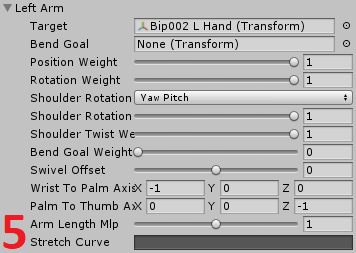
\includegraphics[width=0.35\linewidth]{Bilder/A36_TargetsBendGoals2}
	\caption{Die Inspektor-Ansicht vom VR IK Skript: Target und Bend Goal am Beispiel des linken Arms, eigene Abbildung}
	\label{fig:TargetBendGoal}
\end{figure}
\newline
Des Weiteren enthält das Objekt Dummy mit dem VR IK Skript zwei weitere Kind-Objekte (Vgl. Abbildung \ref{fig:Dummy}), den \textbf{BipDummy} und den gleichnamigen \textbf{Dummy}. Letzterer ist nur der Skinned-Mesh-Renderer und kümmert sich darum, dass die Texturen der Körperteile gerendert werden. Dies bietet den Vorteil, dass sich das Aussehen des Menschen leicht durch neue Texturen verändern lässt. Das Objekt BipDummy enthält die Transformationen, also Position, Rotation und Skalierung, aller Körperteile. Dieser Modulare Aufbau ermöglicht, das Menschmodell in Zukunft durch beliebige neue Modelle auszutauschen, solange mindestens die Transformationen für die Körperteile Füße, Knie, Steißbein, Hände, Ellenbogen und Kopf vorhanden sind.
\begin{figure}[h]
	\centering
	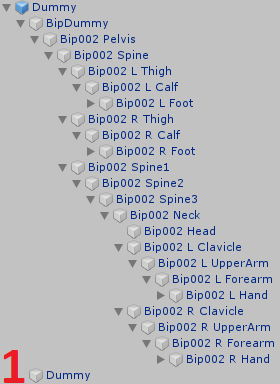
\includegraphics[width=0.35\linewidth]{Bilder/A34_DummyAufbau2}
	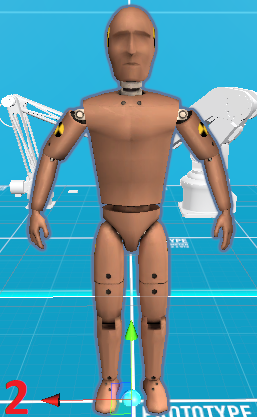
\includegraphics[width=0.296\linewidth]{Bilder/A35_Dummy2}
	\caption{Die Hierarchie- und Szenen-Ansicht vom Final IK Dummy Modell, eigene Abbildung}
	\label{fig:Dummy}
\end{figure}
\newpage

\subsection{Ergänzende Komponenten für das Menschmodell}\label{sec:MMKomponenten}
Das Menschmodell einsatzfähig für die VR Hardware zu machen, erfordert, neben den Skripten, noch zwei weitere Komponenten, die zu dem eigentlichen Modell hinzugefügt werden mussten (Vgl. Abbildung \ref{fig:UnityOverview}). Diese Komponenten sind das SteamVR CameraRig (Kamera) und die Targets (Verfolgungsziele) für die optionalen Tracker.
\newline\newline
Das \textbf{SteamVR CameraRig} (Vgl. Abbildung \ref{fig:CameraRig}), ist eine von SteamVR zur Verfügung gestellte Komponente zur Eingrenzung des Spielbereichs und Tracking der Controller (Hier: Hände) und der VR-Brille (Hier: Kopf). Die Komponente besteht aus den drei Kind-Objekten Controller (left), Controler (right) und Camera. Controller (left) und Controller (right) enthalten zusätzlich ein 3D-Modell des Controllers als Kind-Objekt, um diesen in der virtuellen Welt anzeigen zu können. Durch diese drei Objekte werden die Bewegungen der beiden Hände und des Kopfes in der virtuellen Welt wiedergespiegelt. Des Weiteren ist es wichtig zu erwähnen, dass das CameraRig für diese Arbeit modifiziert wurde. Den beiden Controllern und der Kamera wurden Kopien der Transformationen der beiden Hände und des Kopfes als Kind-Objekte hinzugefügt. Diese Transformationen kamen beim VR IK Skript (Vgl. Abbildung \ref{fig:TargetBendGoal}) zum Einsatz, um Informationen über die Position und Ausrichtung der Hände und des Kopfes zu erhalten, da diese sich als Kind-Objekte der Controller (Hier: Hände) und der Kamera (Hier: Kopf) entsprechend mitbewegen. Abschließend sei noch zu erwähnen, dass die Transformation vom Kopf (Bip002 Head) um -0,113 Einheiten entlang der Y- und Z-Achse gegenüber dem Parent-Objekt Camera verschoben wurde, damit die Kamera sich nicht innerhalb des Kopfes des Modells, sondern auf Höhe der Augen befindet.
\begin{figure}[h]
	\centering
	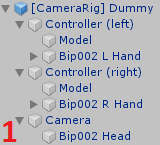
\includegraphics[width=0.25\linewidth]{Bilder/A37_CameraRig2}
	\caption{Die Hierarchie-Ansicht vom modifizierten CameraRig, eigene Abbildung}
	\label{fig:CameraRig}
\end{figure}
\newline
Die zweite wichtige Komponente sind die sogenannten \textbf{Targets} (Vgl. Abbildung \ref{fig:Targets}). Da nur sichergestellt ist, dass der Kopf und die Hände durch die VR-Brille und die Controller, mit Hilfe des SteamVR CameraRigs, verfolgt werden, bedarf es zusätzliche Verfolgungsziele für die optionalen Tracker an den Füßen, Knien, Ellenbogen und dem Steißbein. Die Targets enthalten momentan noch jeweils ein Kind-Objekt (Vgl. Abbildung \ref{fig:Targets}), welches lediglich für den Entwicklungsprozess gedacht ist und auf Wunsch einfach gelöscht werden kann, da es sich nur um eine einfache gefärbte Kugel handelt, die dem Entwickler anzeigt, wo der Tracker sich momentan im Raum befinden. Des Weiteren kommen die Targets, genauso wie die Transformationen der Hände und des Kopfes im CameraRig, beim VR IK Skript zum Einsatz, um dem Skript Informationen über die Position und Ausrichtung der entsprechenden Körperteile zu liefern. Dabei ist anzumerken, dass die Füße als Targets zum Einsatz kommen, während das Steißbein, die Knie und die Ellenbogen als Bend Goals verwendet werden (Vgl. Abbildung \ref{fig:TargetBendGoal}).
\begin{figure}[h]
	\centering
	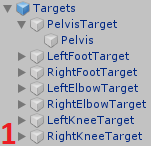
\includegraphics[width=0.25\linewidth]{Bilder/A38_Targets2}
	\caption{Die Hierarchie-Ansicht der Targets, eigene Abbildung}
	\label{fig:Targets}
\end{figure}
\newline
Jedes der angesprochenen Targets enthält, wie bereits in Abbildung \ref{fig:CodeDarstellung} illustriert, das Skript \textbf{SteamVR\_TrackedObject} (Vgl. Abbildung \ref{fig:TrackedObject}). Durch das bereits erwähnte Skript TrackerAssignment, wird jedem der Targets der Index des zugehörigen Trackers zugewiesen. Die Standardeinstellung ist „none“, da das Menschmodell auch ohne jegliche dieser optionalen Tracker und sogar nur mit einer beliebigen Teilmenge von ihnen funktioniert.
\begin{figure}[h]
	\centering
	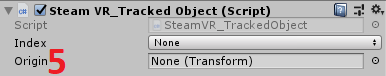
\includegraphics[width=0.45\linewidth]{Bilder/A39_SteamVRTrackedObject2}
	\caption{Die Inspektor-Ansicht vom SteamVR\_TrackedObject Skript, eigene Abbildung}
	\label{fig:TrackedObject}
\end{figure}

\subsection{Skripte für das Menschmodell}\label{sec:MMCode}
Für das eigentliche Menschmodell, ohne die Interaktionsschnittstelle, kommen wie bereits in Abbildung \ref{fig:CodeDarstellung}  und \ref{fig:UnityOverview} dargestellt, zwei weitere Skripte zum Einsatz. Diese beiden Skripte tragen die Namen CalibrationController und TrackerAssignment und befinden sich, genauso wie das CameraRig, der Dummy und die Targets, als Kind-Objekte vom Menschmodell (Human) in der Szene (Vgl. Abbildung \ref{fig:UnityOverview}).
\newline\newline
Das Skript \textbf{TrackerAssignment} (Vgl. Abbildung \ref{fig:MenschUML}) kümmert sich um die Zuweisung der Tracker zu den entsprechenden Körperteilen. Aufgrund dessen enthält dieses Skript in öffentlichen Variablen Verweise auf alle SteamVR Tracked Object Skripte der optionalen Tracker, sowie die Transformationen der zugehörigen Körperteile. Des Weiteren enthält dieses Skript in öffentlichen Variablen Verweise auf das Skript CalibrationController und das VR IK Skript vom Dummy. Außerdem enthält dieses Skript noch einige private Variablen, insbesondere die bereits in Kapitel \ref{sec:Variablendefinition} erwähnten IDs der verschiedenen Tracker.
\newline
Insgesamt enthält das Skript zwei Methoden. Die erste Methode trägt den Namen Start und wird einmalig bei der Initialisierung und danach nie wieder ausgeführt. In dieser Methode werden lediglich ein paar Variablen, die im späteren Verlauf verwendet werden, initialisiert. Die zweite Methode trägt den Namen AssignTrackers und beinhaltet die gesamte Funktionalität dieses Skripts.
In der Methode AssignTrackers werden zunächst, mittels einer Schleife alle, angeschlossenen Geräte durchlaufen und mit den hinterlegten IDs der Tracker verglichen. Sobald die ID von einem der angeschlossenen Geräte, mit einer der hinterlegten IDs übereinstimmt, wird dem SteamVR Tracked Object Skript des Targets des entsprechenden Körperteils, der Index dieses Trackers zugewiesen (Vgl. Abbildung \ref{fig:TrackedObject}). Dies ist notwendig, da die Tracker bei jeder neuen Verbindung mit dem PC einen zufälligen Index zwischen eins und 16 erhalten.
Daraufhin werden dem Calibration Controller die Referenzen zu den Transformationen der Füße und des Steißbeins übergeben (Vgl. Abbildung \ref{fig:CodeDarstellung}), falls die entsprechenden Tracker aktiv sind. In diesem Fall setzt der Calibration Controller automatisch die Füße als Targets und das Steißbein als Bend Goal im VR IK Skript ein. Es ist anzumerken, dass jede beliebige Teilmenge dieser drei Tracker aktiv sein kann, da die Kalibrierung auch nur mit Hilfe der Positionen der Hände und des Kopfes durchgeführt werden kann.
Anschließend werden, durch den Verweis auf das VR IK Skript, die übrigen Bend Goals zugewiesen, falls die Tracker für die Knie und Ellenbogen angeschlossen sind. Dafür muss zusätzlich das Bend Goal Weight (die Gewichtung des Bend Goals) auf den Wert 1 gesetzt werden (Vgl. Abbildung \ref{fig:TargetBendGoal}). Hier ist ebenfalls anzumerken, dass jede beliebige Teilmenge dieser Tracker aktiv sein kann, ohne das Ergebnis der Darstellung des Menschmodells wesentlich zu verschlechtern. Falls beispielsweise der Tracker am linken Ellenbogen aktiv ist, aber der Tracker am rechten Ellenbogen nicht, wird die Position des rechten Ellenbogens einfach durch das VR IK Skript, anhand der Positionen und Ausrichtungen der rechten Hand und des restlichen Körpers, automatisch approximiert.
\newline\newline
Das Skript \textbf{CalibrationController} (Vgl. Abbildung \ref{fig:MenschUML}) arbeitet mit dem bereits vorhandenen VR IK Calibrator des Final IK Plugins. Aufgrund dessen enthält das Skript in öffentlichen Variablen die Verweise auf das VR IK Skript vom Dummy, auf die Transformationen vom Kopf und den beiden Händen und auf das Skript TrackerAssignment. Des Weiteren enthält das Skript die öffentlichen Variablen Settings (Einstellungen) und Data (Daten der Kalibrierung). Schließlich enthält das Skript noch öffentlich deklarierte, aber noch nicht initialisierte, Variablen für die Verweise auf die Transformationen des Steißbeins und der beiden Füße.
\newline
Insgesamt enthält das Skript drei Methoden, wobei die letzte den Namen LateUpdate trägt und in der Regel nicht verwendet wird. Diese Methode ist nur für Entwicklungszwecke da und war bereits in einer Demo-Klasse des Final IK Plugins vorhanden. Sie ermöglicht es einem, die Kalibrierung des Dummys durch das drücken einer bestimmten Taste auf der Tastatur zu starten. Die erste Methode dieses Skripts trägt den Namen Update und wird einmal pro Frame ausgeführt. Aufgabe dieser Methode ist es, sobald vom Bediener die entsprechende Taste am linken Controller gedrückt wird, den Kalibrierungsprozess durch Aufruf der zweiten Methode des Skripts, mit dem Namen Calibrate, zu starten. Es ist anzumerken, dass der Kalibrierungsprozess beliebig oft ausgeführt und somit die Kalibrierung nach Bedarf erneuert werden kann.
In der Methode Calibrate wird zunächst durch den Verweis auf das Skript TrackerAssignment die Zuweisung der einzelnen Tracker gestartet. Hierbei ist anzumerken, dass wie bereits vorher erwähnt und in Abbildung \ref{fig:CodeDarstellung} dargestellt, die noch nicht initialisierten Variablen für die Verweise auf die Transformationen des Steißbeins und der beiden Füße initialisiert werden, falls die entsprechenden Tracker angeschlossen sind. Ansonsten werden für die Kalibrierung lediglich die Positionen der Hände und des Kopfes berücksichtigt. In jedem Fall werden für die Kalibrierung die Positionen der Knie, der Ellenbogen und des Steißbeins nicht berücksichtigt.
Schließlich wird der eigentliche Kalibrierungsprozess durch die gleichnamige Methode Calibrate des Skripts VR IK Calibrator gestartet, indem die entsprechenden Variablen an diese Methode übergeben werden. Die vorher angesprochenen Variablen Settings und Data sind dafür da, falls mit Hilfe der Klasse VR IK Calibrator und deren Methoden Kalibrierungen abgespeichert und wieder geladen werden sollen. Diese Funktionalität wurde für diese Arbeit nicht berücksichtigt.
\begin{figure}[h]
	\centering
	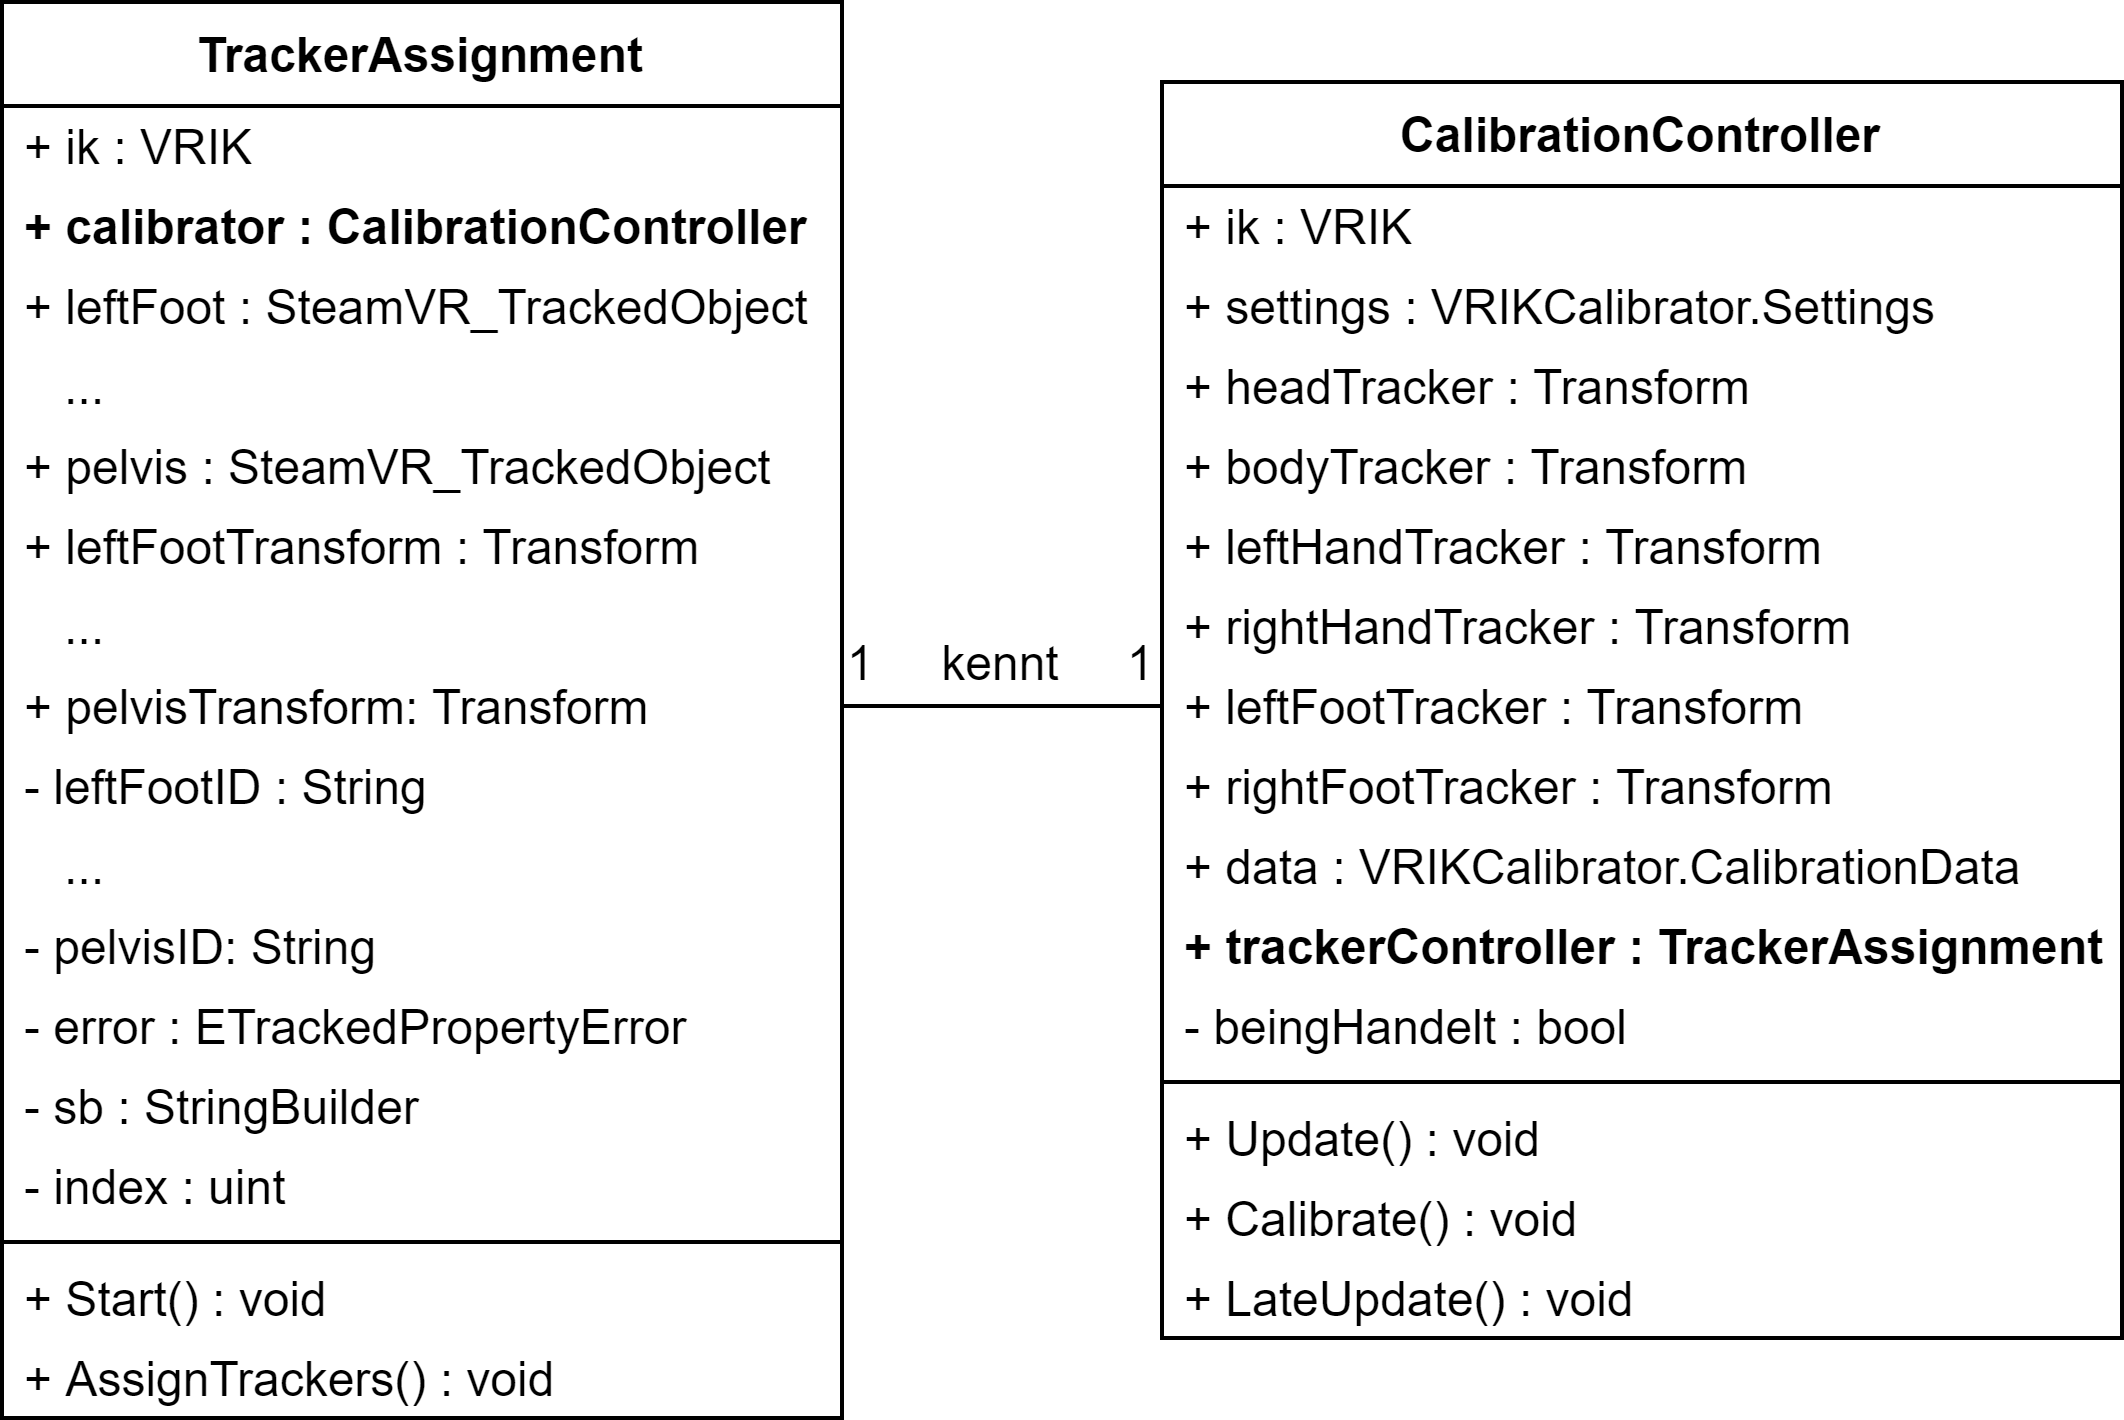
\includegraphics[width=0.6\linewidth]{Bilder/A40_MenschUML}
	\caption{Das UML Diagramm der Skripte für das Menschmodell, eigene Abbildung}
	\label{fig:MenschUML}
\end{figure}

\subsection{Das fertige Menschmodell}\label{sec:MMFunktionen}
Das entstandene Menschmodell, welches auf dem Modell eines Crashtest-Dummys aus dem Final IK Plugins basiert, ermöglicht, in Verbindung mit der SteamVR Schnittstelle und der entsprechenden Hardware, die Abbildung der Bewegungen des Bedieners auf einen virtuellen Klon. Dabei müssen mindestens die VR Brille und die Controller verwendet werden, um mittels der Positionen der Hände und des Kopfes die Bewegungen des Bedieners abbilden zu können. Falls nur die VR Brille und die Controller verwendet werden, werden die Bewegungen der restlichen Körperteile durch das VR IK Skript approximiert. Des Weiteren ermöglicht dieses Menschmodell, mit Hilfe der in Abbildung \ref{fig:Mounts} dargestellten Befestigungen, den Einsatz der HTC VIVE Tracker, um die Bewegungen der Füße, der Knie, der Ellenbogen und des Steißbeins zu berücksichtigen und somit ein genaueres virtuelles Abbild der Bewegungen zu erhalten. Es ist anzumerken, dass nicht jeder dieser Tracker aktiv sein muss und sogar jede beliebige Teilmenge dieser optionalen Tracker aktiv sein kann, da Bewegungen von Körperteilen die nicht verfolgt werden, wie bereits erwähnt, durch das VR IK Skript approximiert werden.
\newline
Schließlich ist noch wichtig zu erwähnen, dass das entstandene Menschmodell in der Szene lediglich aus den Objekten '[CameraRig] Dummy' (die SteamVR Kamera), 'Dummy' (das eigentliche Modell), 'HumanScripts' (die beiden Skripte) und 'Targets' (die Verfolgungsziele) besteht (Vgl. Abbildung \ref{fig:UnityOverview}).

%--------------------------------------------------------------------------------------------------
\section{Die Interaktionsschnittstelle}\label{sec:DieInteraktionsschnittstelle}
Einerseits ist das Menschmodell nützlich, um die Bewegungen des Bedieners in der virtuellen Welt, also beispielsweise in der virtuellen Produktionsanlage, abzubilden, andererseits fehlt dem Menschmodell noch die Möglichkeit, mit der virtuellen Umgebung zu interagieren. Daher wird in diesem Abschnitt der Aufbau und der Nutzen der Interaktionsschnittstelle erläutert. Die Grundidee der Interaktionsschnittstelle ist es, das Menschmodell durch einen Pointer (Zeiger) zu erweitern und somit eine intuitive Interaktion mit der Umgebung zu ermöglichen (Vgl. Abbildung \ref{fig:InteraktionBeispiel}).
\begin{figure}[h]
	\centering
	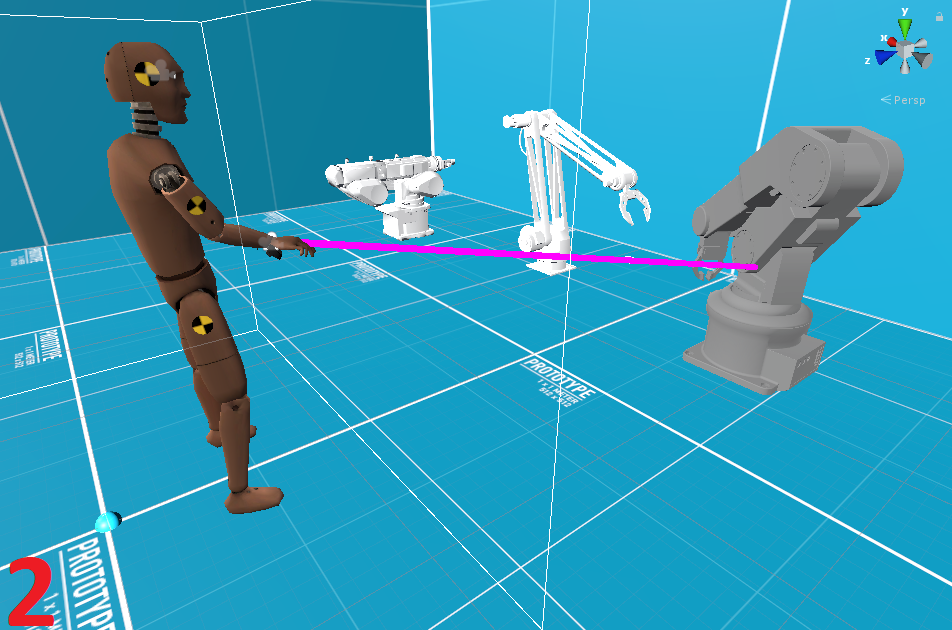
\includegraphics[width=0.6\linewidth]{Bilder/A44_InteraktionsBeispiel2}
	\caption{Die Szenen-Ansicht der Grundidee der Interaktion, eigene Abbildung}
	\label{fig:InteraktionBeispiel}
\end{figure}
\newline
\noindent Im Folgenden wird zunächst das Grundgerüst der Interaktionsschnittstelle erklärt, bevor die zusätzlichen Funktionalitäten erläutert werden. Es ist anzumerken, dass die zusätzlichen Funktionalitäten nur hinzugefügt wurden, um ein Anwendungsbeispiel für die Interaktionsschnittstelle zu schaffen und somit ihren Nutzen hervorzuheben.

\subsection{Das Grundgerüst der Interaktionsschnittstelle}\label{sec:GrundgerüstInteraktion}
Das Grundgerüst der Interaktionsschnittstelle besteht lediglich aus dem Interaktionssystem, den beiden Pointern, dem Skript für den Wechsel zwischen den beiden Pointern und dem Skript für das aufrufen des Menüs des angeklickten Objekts. Es ist anzumerken, dass zwei Pointer verwendet wurden, da der eine Pointer genutzt wird um mit Objekten in der Umgebung, wie z.B. Robotern, zu interagieren, während der andere Pointer dafür da ist, um mit graphischen Benutzeroberflächen zu interagieren. Außerdem ist anzumerken, dass die Klassen VR Input für das Interaktionssystem und VR Canvas Pointer und VR Physics Pointer für die beiden Pointer auf Anleitungen des YouTube Kanals 'VR with Andrew' basieren \cite{32}. Sowohl das Interaktionssystem, als auch das Skript für den Wechsel zwischen den Pointern, befinden sich in der Szene. Das Interaktionssystem in der Szene trägt den Namen 'EventSystem with VR Input', während das Skript für den Wechsel zwischen den Pointern bestandteil des Objekts 'Scripts' ist. Beide sind Kindobjekte vom Objekt 'InteractionEventSystemAndScripts' (Vgl. Abbildung \ref{fig:UnityOverview}). Im Gegensatz dazu, befindet sich keiner der beiden Pointer vor Ausführung des Programms in der Szene. Eine genauere Erläuterung der Pointer folgt im weiteren Verlauf dieses Kapitels.
\newline\newline
Das \textbf{Interaktionssystem} (Vgl. Abbildung \ref{fig:EventSystem}) basiert auf dem sogenannten Event System von Unity, welches standardmäßig in jeder Szene vorhanden ist. Mit Hilfe des Event Systems wird in der Regel der Input der Tastatur und der Maus gehandhabt. Das Event System wird für diese Arbeit durch das Skript \textbf{VR Input} (Vgl. Abbildung \ref{fig:UMLInteraktion}) erweitert, welches die drei öffentlichen Variablen eventCamera, clickButton und clickAction enthält. Die Variable eventCamera erhält bei Ausführung des Programms einen Verweis auf die Kamera des aktuell genutzten Pointers, während die Variablen clickButton und clickAction lediglich genutzt werden, um die Input-Taste zu deklarieren. Für diese Arbeit wird die Taste auf der Rückseite des rechten Controllers als Input-Taste verwendet.
\newline
Insgesamt enthält das Skript fünf Methoden. Die erste Methode trägt den Namen Awake, dient lediglich zur Initialisierung und wird automatisch ausgeführt sobald eine der Methoden in der Klasse ausgeführt wird. Es ist anzumerken, dass für den Input der VR Hardware der Input der Maus überschrieben wird. Daher haben die übrigen vier Methoden die Aufgabe, den Input der Maus zu überschreiben. Die erste dieser vier Methoden trägt den Namen GetMouseButton und liefert Informationen darüber, ob die Taste gedrückt und wieder losgelassen wurde, während die Methoden GetMouseButtonDown und GetMouseButtonUp dem Entwickler ermöglichen separat abzufragen, ob die Taste runter gedrückt oder losgelassen wurde. Die letzte Methode des Skripts trägt den Namen mousePosition und überschreibt die Position der Maus durch den exakten Mittelpunkt der aktuellen EventCamera. Somit wird durch das Klicken der Input-Taste am rechten Controller das Klicken mit der Maus simuliert.
\begin{figure}[h]
	\centering
	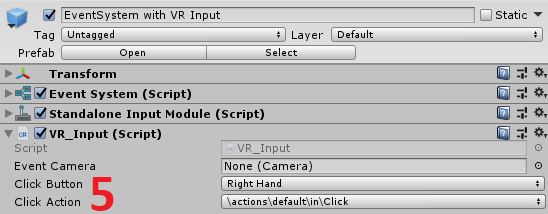
\includegraphics[width=0.5\linewidth]{Bilder/A41_EventSystem2}
	\caption{Die Inspektor-Ansicht vom Event System mit VR Input, eigene Abbildung}
	\label{fig:EventSystem}
\end{figure}
\newline
Sowohl der \textbf{Canvas Pointer} (Vgl. Abbildung \ref{fig:UMLInteraktion}) als auch der \textbf{Physics Pointer} (Vgl. Abbildung \ref{fig:UMLInteraktion}) enthalten die Komponenten Camera (Kamera), Line Renderer (Linien zeichner) und das zugehörige Skript. Der Physics Pointer enthält zusätzlich die Komponente Physics Raycaster (Vgl. Abbildung \ref{fig:Pointer}). Mit Hilfe der Komponente Camera lässt sich bestimmen, worauf der aktuelle Pointer zeigt, da wie bereits erwähnt, der Mittelpunkt der Kamera genommen wird, um den Maus Input zu überschreiben. Diese Komponente wird durch das im späteren Verlauf dieses Kapitels vorgestellte Skript Switch Pointers beim Event System hinterlegt (Vgl. Abbildung \ref{fig:EventSystem}). Der Line Renderer hat lediglich die Aufgabe, eine Linie zu zeichnen, damit der Bediener erkennen kann, worauf er zeigt/klickt. Diese Linie beginnt beim Controller in der rechten Hand des Bedieners und ist standardmäßig drei Unity-Einheiten lang. Falls ein Objekt die Linie schneidet, endet diese an dem Schnittpunkt. 
\newline
Grundsätzlich funktionieren die Skripte VR Physics Pointer und VR Canvas Pointer nach dem gleichen Prinzip. Es wird ausgehend vom Ursprung des Pointers ein Raycast (Strahl) gesendet und anschließend überprüft womit dieser kollidiert. Der Unterschied zwischen den beiden Pointern ist, dass durch das Skript VR Physics Pointer ein Raycast gesendet wird, der nur mit Objekten die einen Collider (Kollisions-Box) besitzen kollidieren kann (Physics Raycast). Im Gegensatz dazu sendet das Skript VR Canvas Pointer mit Hilfe des Event Systems einen Raycast, der nur mit Objekten die Bestandteil einer graphischen Benutzeroberfläche sind, kollidieren kann. Aufgrund dessen gibt es zwei Anforderung an die Umgebung. Erstens müssen alle Objekte mit denen interagiert werden soll einen Collider besitzen, sodass diese mit dem Physics Pointer angeklickt werden können. Zweitens müssen die Menüs dieser Objekte die bereits in Unity vorhandenen Elemente wie, beispielsweise Knöpfe oder Slider, für die Implementierung ihrer grafischen Benutzeroberflächen benutzen.
\newline
Der aktuell eingesetzte Pointer in wird, sobald das Programm ausgeführt wird, als Kind-Objekt des rechten Controllers (Vgl. Abbildung \ref{fig:UnityOverview}), instanziiert. Somit bewegt sich der Pointer mit der rechten Hand, beziehungsweise mit dem rechten Controller mit und ermöglicht eine intuitive Interaktion mit der Umgebung. Zu Beginn wird Standardmäßig der Physics Pointer instanziiert, sobald jedoch ein Objekt angeklickt wird und sich somit das Menü dieses Objektes öffnet, wird auf den Canvas Pointer gewechselt. Des Weiteren ist anzumerken, dass sobald das aktuell geöffnete Menü geschlossen wird, auf den Physics Pointer zurück gewechselt wird.
\begin{figure}[h]
	\centering
	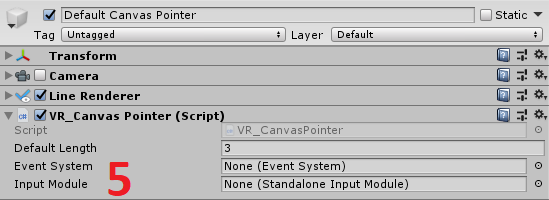
\includegraphics[width=0.49\linewidth]{Bilder/A42_CanvasPointer2}
	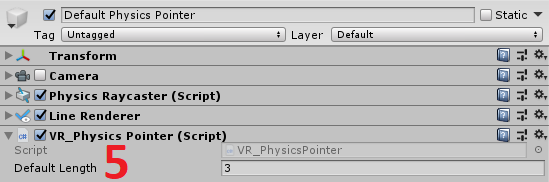
\includegraphics[width=0.49\linewidth]{Bilder/A43_PhysicsPointer2}
	\caption{Die Inspektor-Ansicht vom Canvas und Physics Pointer, eigene Abbildung}
	\label{fig:Pointer}
\end{figure}
\newline
Wie bereits erwähnt, wird der zwischen den Pointern durch das Skript \textbf{Switch Pointers} (Vgl. Abbildung \ref{fig:UMLInteraktion}) gehandhabt. Dieses enthält in öffentlichen Variablen Verweise auf die Objektvorlagen der beiden Pointer (Vgl. Abbildung \ref{fig:SwitchPointer}), damit diese bei Ausführung des Programms als Kind-Objekte des rechten Controllers instanziiert werden können.
\newline
Zu Beginn wird in der Methode Start ein Physics Pointer instanziiert, dessen Kamera Komponente als Event Camera beim Event System gesetzt wird (Vgl. Abbildung \ref{fig:EventSystem}). Durch die Methode Update wird die Methode HandlePointerSwitch jede Sekunde mehrfach aufgerufen. Sobald ein Objekt angeklickt wird und sich sein Menü öffnet, wird der Pointer mit Hilfe der Methode HandlePointerSwitch ausgetauscht und die Event Camera beim Event System entsprechend aktualisiert. Des Weiteren werden bei dem Canvas Pointer die Referenzen zum Event System und seinem Input Module gesetzt (Vgl. Abbildung \ref{fig:Pointer}). Instanziiert werden die Pointer mittels der beiden Hilfsmethoden SpawnPhysicsPointer und SpawnCanvasPointer.
\begin{figure}[h]
	\centering
	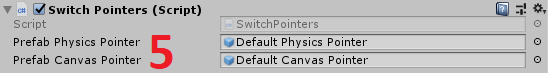
\includegraphics[width=0.6\linewidth]{Bilder/A45_SwitchPointer2}
	\caption{Die Inspektor-Ansicht von Switch Pointers, eigene Abbildung}
	\label{fig:SwitchPointer}
\end{figure}
\newline
Die letzte Komponente des Grundgerüsts der Interaktionsschnittstelle ist das Skript \textbf{Object Menu} (Vgl. Abbildung \ref{fig:UMLInteraktion}), welches zu jedem beliebigen Objekt in der Szene hinzugefügt werden kann, solange dieses Objekt über einen Collider verfügt. Sobald das Skript zu einem Objekt hinzugefügt wird, taucht des in der Inspektor-Ansicht des jeweiligen Objekts auf. Dabei sind die wichtigsten Komponenten dieses Skripts die öffentlichen Variablen prefab, thisObject, clickButton und clickAction (Vgl. Abbildung \ref{fig:ObjectMenu}). Die Variable prefab enthält den Verweis auf die Objektvorlage des zu öffnenden Menüs, während die Variable thisObject den Objektverweis auf das Objekt, zu dem das Skript gehört, enthält. Wie bereits beim Interaktionssystem werden die Variablen clickButton und clickAction benutzt, um die Input-Taste (für das Schließen des Menüs) zu deklarieren. Für diese Arbeit werden standardmäßig die Tasten auf der Außenseite des rechten Controller zum schließen von Menüs verwendet. Daher muss der Controller fest in der Hand gedrückt werden, um das Menü zu schließen.
\newline
Insgesamt enthält das Skript vier Methoden. In der Methode Start werden lediglich einige private Hilfsvariablen deklariert. Durch die Methode Update wird in jeder Sekunde mehrmals überprüft, ob ein Objekt angeklickt wurde und ein Menü geöffnet werden soll. Dabei hat die Methode ClickHandler die Aufgabe, eine private Hilfsvariable zu setzen sobald ein Objekt angeklickt wurde und das Menü geöffnet werden soll. In diesem Fall wird die Methode HandleButtonPress aufgerufen, welche dann eine Instanz des zu öffnenden Menüs instanziiert. Beim erneuten aufrufen der Methode HandleButtonPress, durch das Drücken der angesprochenen Taste am rechten Controller, wird das bereits geöffnete Menü wieder geschlossen. Des Weiteren aktualisiert die Methode Update die Position des Menüs mehrmals pro Sekunde, sodass sich das Menü mit der Kopfbewegung des Bediener mitbewegt und stehts gut sichtbar ist.
\begin{figure}[h]
	\centering
	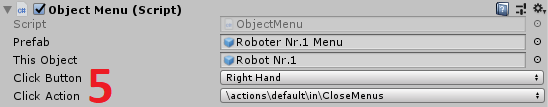
\includegraphics[width=0.6\linewidth]{Bilder/A46_ObjectMenu2}
	\caption{Die Inspektor-Ansicht von Object Menu, eigene Abbildung}
	\label{fig:ObjectMenu}
\end{figure}
\begin{figure}[h]
	\centering
	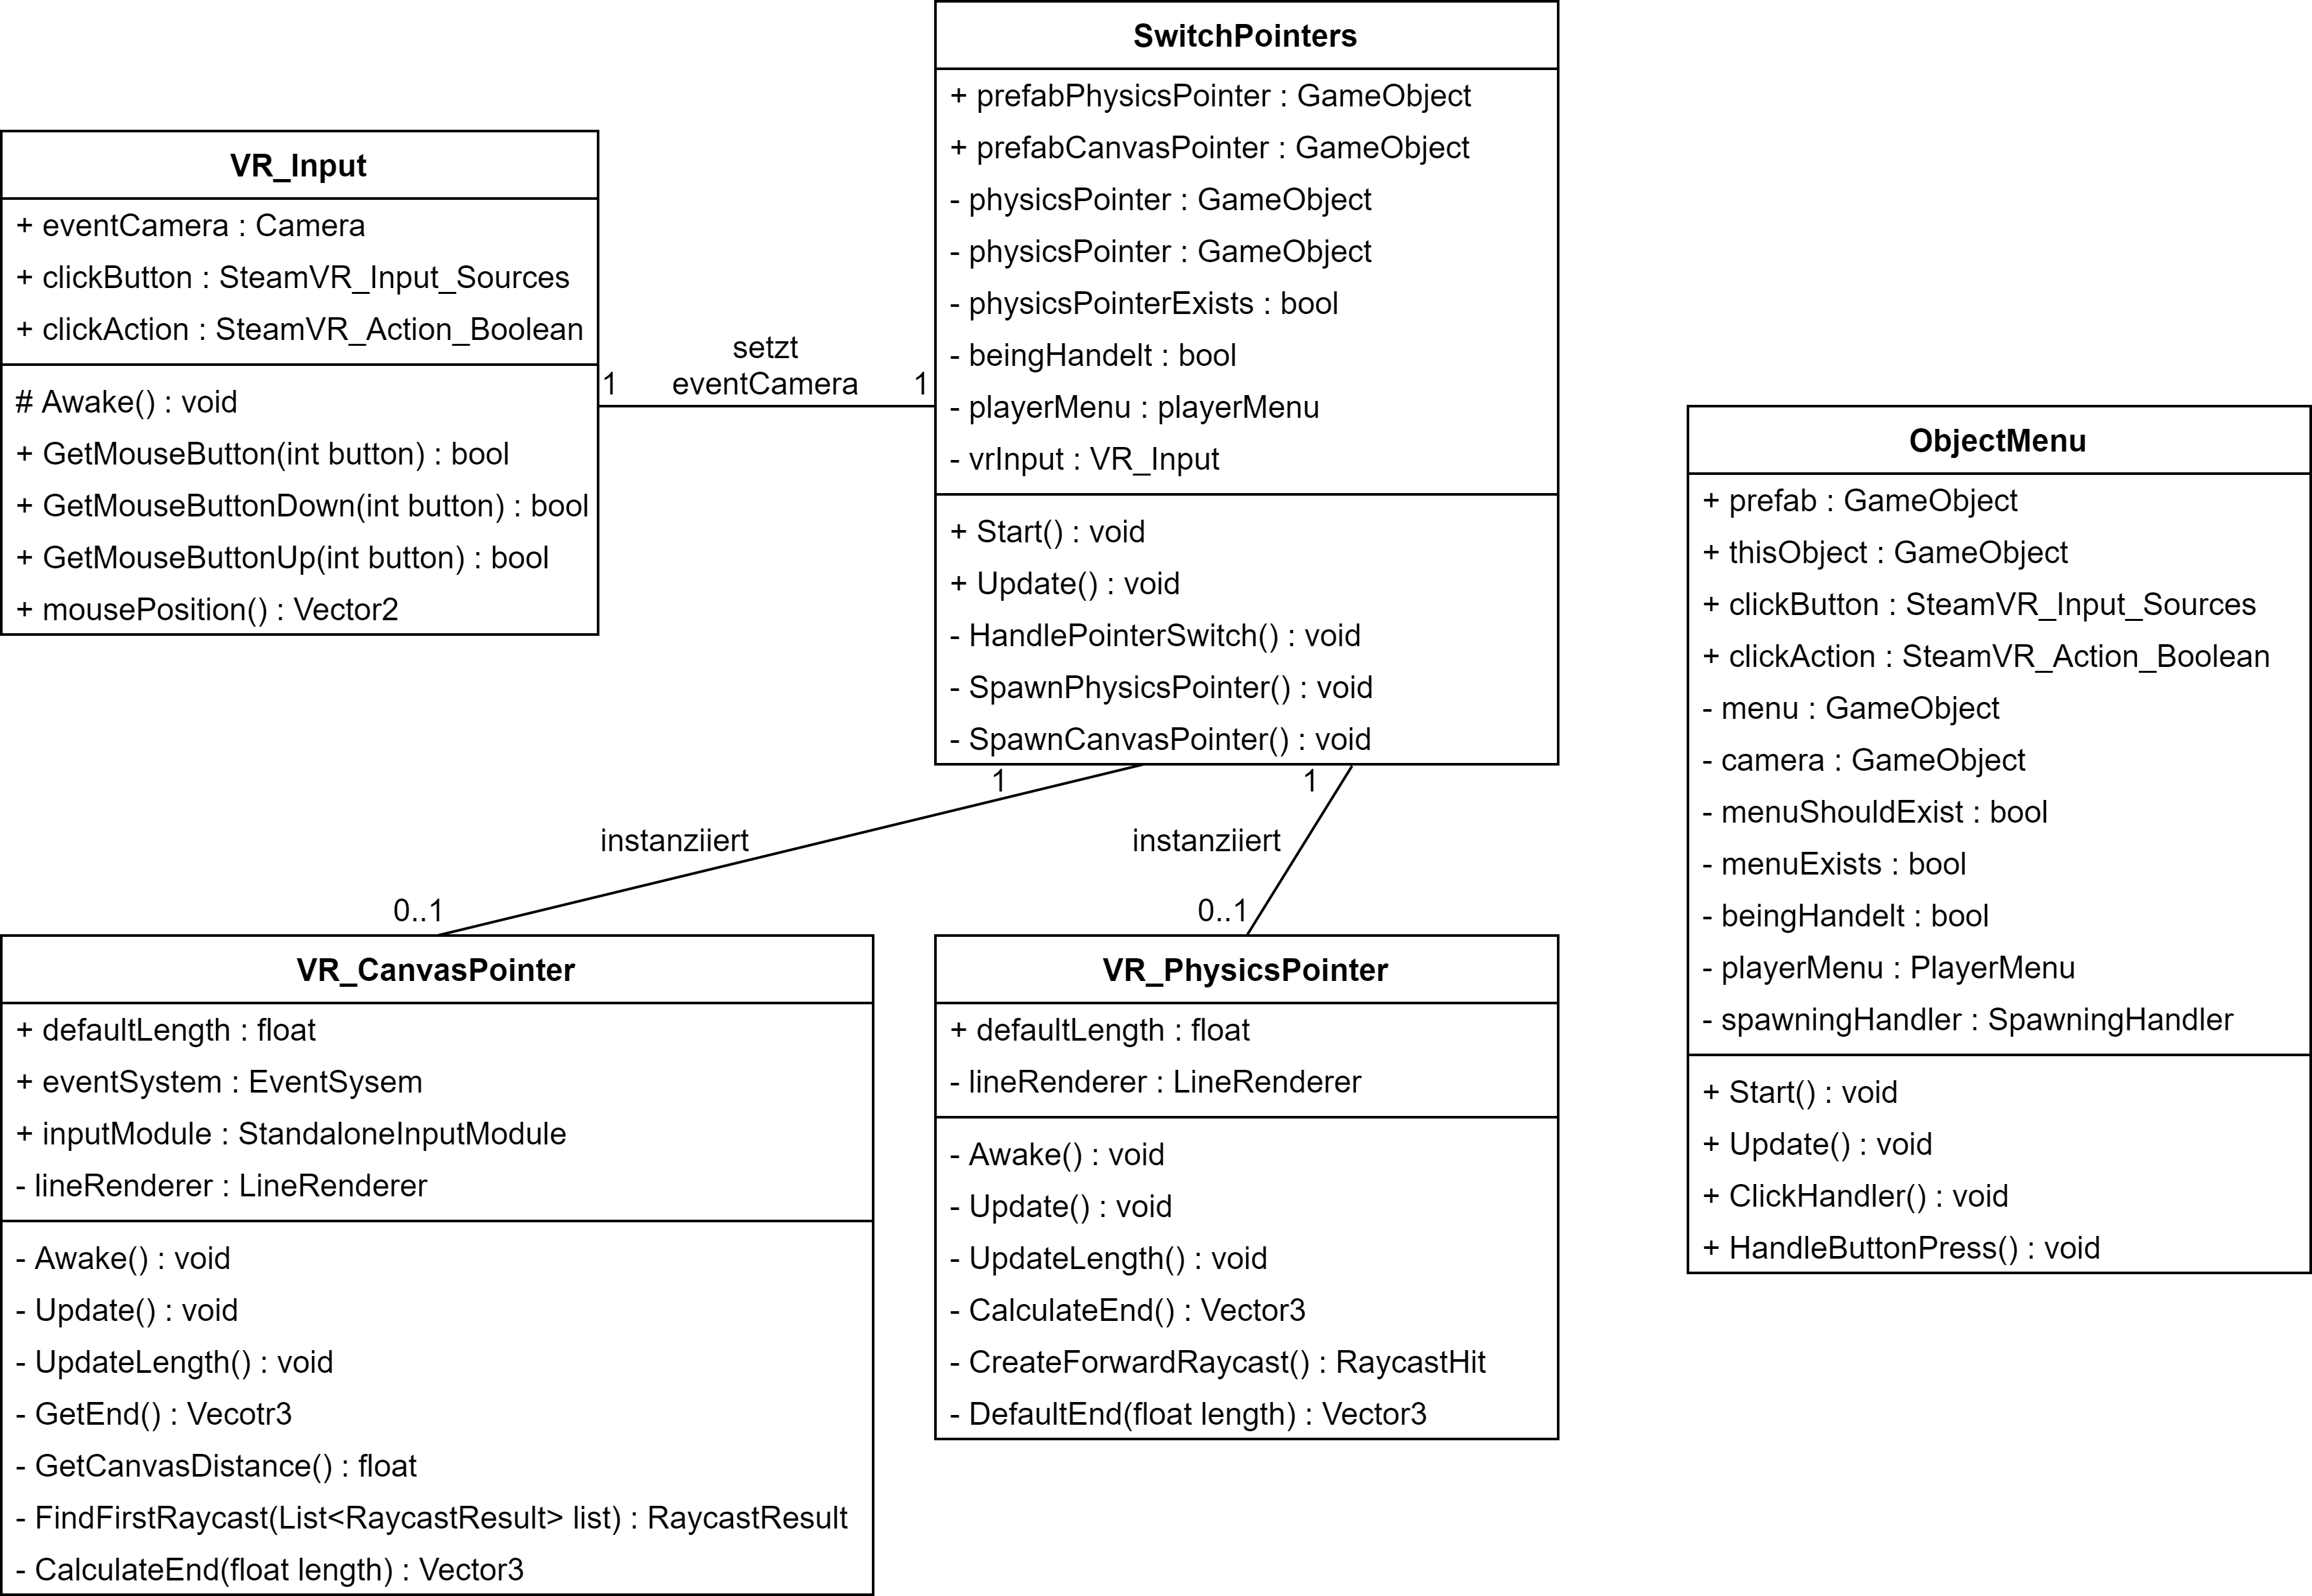
\includegraphics[width=1\linewidth]{Bilder/A48_InteraktionUML1}
	\caption{Das UML Diagramm des Grundgerüsts der Interaktionsschnittstelle, eigene Abbildung}
	\label{fig:UMLInteraktion}
\end{figure}

\subsection{Weitere Bestandteile der Interaktionsschnittstelle}\label{sec:WeitereTeileInteraktion}
Basierend auf dem im vorherigen Abschnitt erläuterten Grundgerüst, werden in diesem Abschnitt zusätzliche Bestandteile der bei dieser Arbeit entstandenen Interaktionsschnittstelle erläutert. In Zukunft könnten die folgenden Bestandteile nach Bedarf ausgetauscht oder verbessert werden, daher wird der Aufbau des Codes der einzelnen Bestandteile im Folgenden nicht im Detail erläutert. Mit Hilfe dieser zusätzlichen Bestandteile soll ein Anwendungsbeispiel für die Interaktionsschnittstelle geschaffen werden, um somit den Nutzen zu demonstrieren.
\newline\newline
Ein zentraler Bestandteil der Interaktionsschnittstelle ist das Hauptmenü, welches durch das Klicken der obersten Taste am rechten Controller durch das Skript Player Menu aufgerufen wird. Das Skript \textbf{Player Menu} ist Bestandteil des Objekts Scripts aus der Szene, welches in Abbildung \ref{fig:UnityOverview} dargestellt ist. Das Hauptmenü wurde hinzugefügt, um einen Anwendungsfall der Interaktionsschnittstelle zu demonstrieren und somit ihren Nutzen hervorzuheben. Insgesamt besteht das Hauptmenü aus drei Benutzeroberflächen (Vgl. Abbildung \ref{fig:MainMenu}). Die erste Benutzeroberfläche ist die Startseite des Hauptmenüs und zeigt dem Bediener den aktuellen Batteriestatus der benutzten Hardware an. Auf die zweite Benutzeroberfläche des Hauptmenüs gelangt der Bediener durch das anklicken des Knopfes „Options“. Hier können durch den Entwickler Einstellungsmöglichkeiten, wie z.B. die maximale Anzahl bestimmter Roboter in einer Produktionsanlage, festgelegt werden. Die letzte Benutzeroberfläche ist das Inventar und wird durch das Anklicken des Knopfes „Inventory“ aufgerufen. Sie bietet dem Entwickler die Möglichkeit, ein Inventar zu implementieren, über welches Produktionsanlagen in den Produktionsräumen platziert werden können. Für diese Arbeit wurden zu Demonstrationszwecken vier Roboter, stellvertretend für Elemente einer Produktionsanlage, hinzugefügt, welche über das Inventar-Menü in der Umgebung platziert werden können.
\begin{figure}[h]
	\centering
	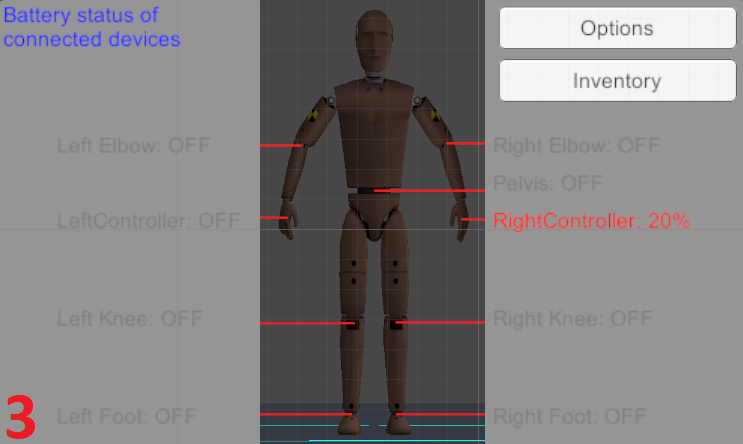
\includegraphics[width=0.45\linewidth]{Bilder/A49_MM1_2}
	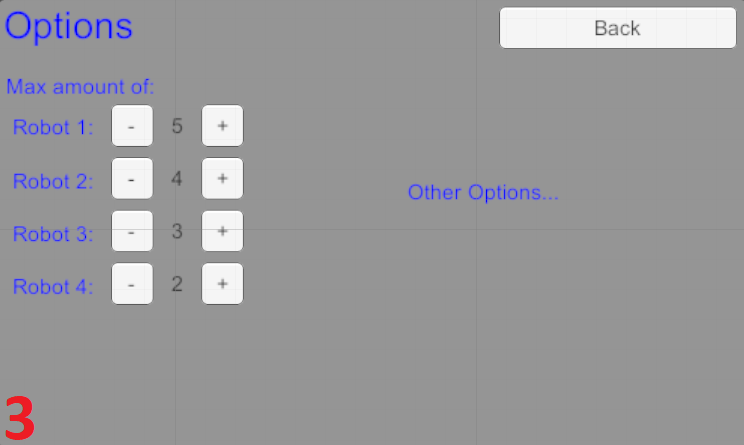
\includegraphics[width=0.45\linewidth]{Bilder/A50_MM2_2}
	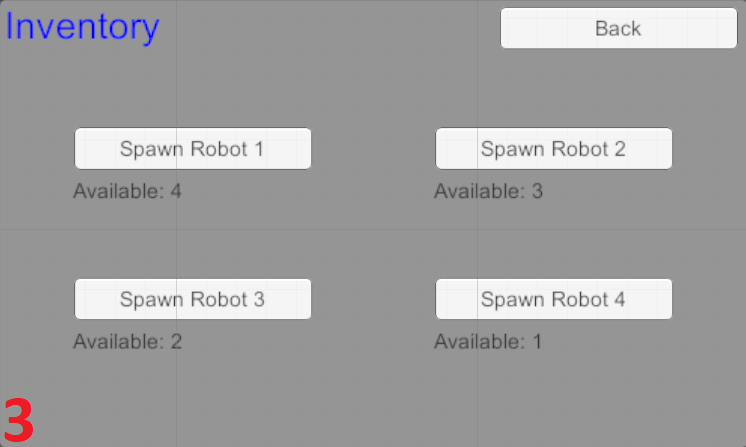
\includegraphics[width=0.45\linewidth]{Bilder/A51_MM3_2}
	\caption{Die Benutzeroberflächen des Hauptmenüs, eigene Abbildung}
	\label{fig:MainMenu}
\end{figure}
\newline
Das Hinzufügen von Robotern in der Szene wird durch die Skripte \textbf{Global Variables} und \textbf{Spawning Handler} ermöglicht. Durch das Skript Spawning Handler werden Roboter instanziiert und in der Szene platziert, sobald dies über das Inventar-Menü durch den Bediener aufgetragen wird. Global Variables hat die Funktion, die aktuelle und maximale Anzahl der Roboter zu verwalten. Des Weiteren verfügt dieses Skript über Referenzen zu den Objektdateien aller vorhandenen Roboter. Damit beispielsweise nicht mehr Roboter von einem Typ, als vorher im Optionen-Menü festgelegt, in der Szene platziert werden können, nutzen Skripte wie Spawning Handler oder auch Player Menu das Skript Global Variables zum synchronisieren. Somit wird sichergestellt, dass wichtige Variablen zentral und für alle Skripte erreichbar verwaltet werden. Sowohl das Skript Spawning Handler, als auch das Skript Global Variables sind Bestandteile des Objekts Scripts aus Abbildung \ref{fig:UnityOverview}.
\newline\newline
Die bereits angesprochenen vier Roboter, die zu Demonstrationszwecken in das Projekt eingefügt wurden (Vgl. Abbildung \ref{fig:UnityOverview}), verfügen alle über ihre \textbf{eigenen Menüs}, welche aus insgesamt zwei Benutzeroberflächen (Vgl. Abbildung \ref{fig:BspMenu}) bestehen. Die erste Benutzeroberfläche kann mit anwendungsspezifischen Funktionalitäten gefüllt werden, während die zweite Benutzeroberfläche bei allen vier Robotern gleich aufgebaut ist. Mit Hilfe der vorhandenen Knöpfe kann der entsprechende Roboter in der virtuellen Produktionsanlage nach Bedarf verschoben oder sogar wieder in das Inventar aufgenommen werden. Es ist anzumerken, dass die Menüs der einzelnen Roboter unabhängig von der Interaktionsschnittstelle sind und daher beliebig viele Benutzeroberflächen beinhalten können. Selbst das Aufnehmen eines Roboters in das Inventar bedarf lediglich den Aufruf einer Methode des Skripts Spawning Handler.
\begin{figure}[h]
	\centering
	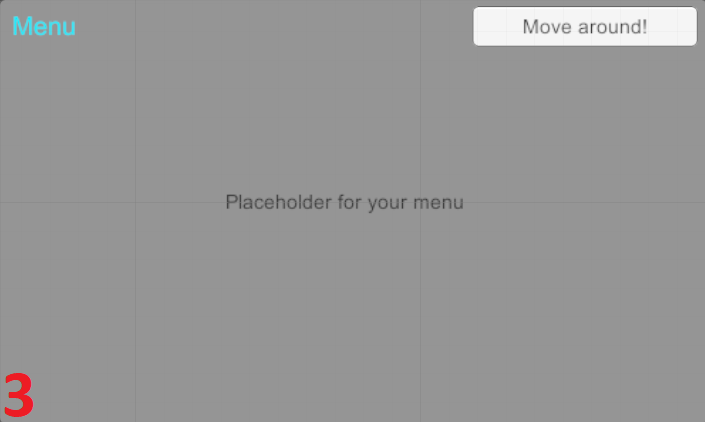
\includegraphics[width=0.45\linewidth]{Bilder/A52_OM1_2}
	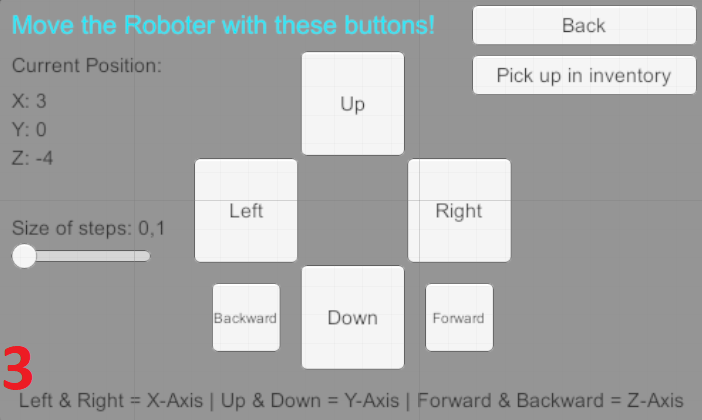
\includegraphics[width=0.45\linewidth]{Bilder/A53_OM2_2}
	\caption{Die Benutzeroberflächen eines exemplarischen Menüs, eigene Abbildung}
	\label{fig:BspMenu}
\end{figure}
\newline
Dem Bediener kann ein optisches Feedback gegeben werden, um somit die Interaktion intuitiver zu gestalten. Daher können bei Bedarf die Skripte \textbf{PointerEvent\_Objects}, für Objekte mit Collidern und \textbf{PointerEvent\_UI}, für Objekte die Bestandteil der graphischen Benutzeroberfläche, sind verwendet werden. Dafür müssen diese Skripte lediglich zu den gewünschten Objekten hinzugefügt werden. Mit Hilfe dieser Skripte verändern Objekte, auf die mit dem Pointer gezeigt wird, ihre Farbe (Vgl. Abbildung \ref{fig:InteraktionBeispiel}). Objekte auf die lediglich gezeigt wird, werden grau gefärbt, sodass der Bediener schnell und intuitiv erkennen kann worauf er gerade zeigt, während angeklickte Objekte rot gefärbt werden, um dem Bediener zu signalisieren, dass das Objekt erfolgreich angeklickt wurde. An dieser Stelle ist anzumerken, dass die Idee für diese Funktionalität vom YouTube Kanal 'VR with Andrew' \cite{32} stammt.
\newpage

\subsection{Die fertige Interaktionsschnittstelle}\label{sec:ZusammenfassungInteraktion}
Durch die entstandene Interaktionsschnittstelle ist der Bediener in der Lage, in der virtuellen Welt sowohl mit Objekten, als auch mit graphischen Benutzeroberflächen zu interagieren. In Verbindung mit dem Menschmodell aus Kapitel \ref{sec:DasMenschmodell}, eröffnen sich viele Anwendungsmöglichkeiten. So könnten beispielsweise Fabrikmitarbeiter, von jedem beliebigem Ort auf der Welt aus, Anlagen einer Fabrik über ihren virtuellen Klon steuern. Dafür Bedarf es jedoch einer entsprechenden Schnittstelle und Infrastruktur, die die virtuelle Welt mit den realen Produktionsanlagen verbindet. Dieses Anwendungsszenario wurde Beispielhaft dargestellt, indem bei dieser Arbeit vier Roboter hinzugefügt wurden, die durch den Bediener in der virtuellen Welt platziert und verschoben werden können. Neben Standortunabhängigkeit ermöglicht dies, die virtuelle Planung von Produktionsanlagen, um Abläufe zu optimieren und somit eine höhere Ressourceneffizienz zu erreichen.
\newline
Schließlich ist noch wichtig zu erwähnen, dass die entstandene Interaktionsschnittstelle lediglich aus einem Objekt in der Szene besteht. Das Objekt trägt den Namen 'InteractionEventSystemAndScripts' und enthält als Kind-Objekte das bereits vorgestellte Interaktionssystem mit dem Namen 'EventSystem with VR Input' und das Objekt 'Scripts', welches alle weiteren nötigen Skripte enthält (Vgl. Abbildung \ref{fig:UnityOverview}). Das mehrfach erwähnte Skript Object Menu ist in der Hierarchie-Ansicht der Szene nicht zu sehen, da es Bestandteil der einzelnen Objekte, wie z.B. Robot Nr.1-4, ist (Vgl. Abbildung \ref{fig:UnityOverview}). Ebenfalls sind der Physics Pointer und der Canvas Pointer nicht in der Hierarchie-Ansicht der Szene vorzufinden, bevor das Programm ausgeführt wird. Erst bei Ausführung des Programms, wird der entsprechende Pointer instanziiert und als Kind-Objekt von 'Controller (right)' in der Szene platziert (Vgl. Abbildung \ref{fig:UnityOverview}).